% ================================================
%   Copyright 2014 Amal Roumi -  Roumia@gmail.com.
%
%    This work is licensed under a Creative Commons 3.0 Unported License.
%    To view a copy of this license visit:
% 
%   http://creativecommons.org/licenses/by-nc-sa/3.0/legalcode
% ================================================

\documentclass[a4paper, 12pt]{book}
\usepackage[a4paper, left=2.5cm, right=2.5cm, top=3cm, bottom=3cm]{geometry}
\setcounter{secnumdepth}{3} %  Numbered Subsubsections
\setcounter{tocdepth}{3} %  adding to the index
\usepackage{indentfirst} %  Indent first paragraph after section header
\usepackage[printonlyused]{acronym}
\usepackage{times}
\usepackage{caption}
\usepackage{color}
\usepackage{eurosym} % for  $
\usepackage{enumitem} % Control layout of itemize, enumerate
\usepackage[usenames,dvipsnames,svgnames,table]{xcolor}
\usepackage[utf8]{inputenc}
\usepackage[textwidth=1cm]{todonotes}
\usepackage[hyphens]{url}
\usepackage[english]{babel}
\usepackage{float}  
\usepackage[nottoc, notlot, notlof, notindex]{tocbibind}
\usepackage{latexsym}  %mathematical symbols
\usepackage{graphicx}
\usepackage[colorlinks,bookmarksopen]{hyperref}
\usepackage{wrapfig}
\urlstyle{rm} % to change the defualt font for the url to rm
\usepackage[compact]{titlesec}  
\captionsetup{textfont={color=NavyBlue},labelfont={color=NavyBlue}}
\usepackage[helvetica]{quotchap}     
\hypersetup{pdftitle={Open source migration },
                     pdfauthor={Amal  Al Roumi},
					 pdfcreator={University Rey Juan Carlos (Madrid, Spain)},
					 pdfproducer=PDFLaTeX,
					 pdfsubject={Master in Software Libre 2013/2014},
				     linkcolor=MidnightBlue,
				     citecolor=OliveGreen,
				     filecolor=violet,
    				 urlcolor=MidnightBlue}
\renewcommand*{\thesubsubsection}{\Alph{subsubsection}}
\frenchspacing
\title{Migrations to Free and Open Source Software: Motivations, Planning and Case Studies}
\author{Amal Roumi}
\renewcommand{\baselinestretch}{1.5}  
%----------------------------------------------------------------
\begin{document}
\renewcommand{\refname}{Bibliography}  
\renewcommand{\appendixname}{Appendix}
%--------------------------------------------------------------------------------------
%TITLE %
%--------------------------------------------------------------------------------------
\begin{titlepage}
\begin{center}
\begin{tabular}[c]{c c}

\includegraphics[scale=0.25]{img/logo.png} &
\begin{tabular}[b]{l}
\Huge
\textsf{UNIVERSIDAD} \\
\Huge
\textsf{REY JUAN CARLOS} \\
\end{tabular}\\
\end{tabular}

\vspace{3cm}

\Large
Master's in Free Software
\vspace{0.4cm}

\large
Academic  year  2013/2014

\vspace{0.8cm}

Final project
\vspace{2.5cm}

\LARGE
Migrations to Free and Open Source Software:\\
Motivations, Planning and Case Studies
\vspace{4cm}

\large
Author: Amal Al Roumi \\
Tutor: Dr. Gregorio Robles
\end{center}
\end{titlepage}
%--------------------------------------------------------------------------------------
%ACKNOWLEDGEMENTS %
%--------------------------------------------------------------------------------------
\newpage
\thispagestyle{empty}
~

\newpage
~
\thispagestyle{empty}
\vspace{3cm}
\begin{flushright}
\textbf{\textit{ACKNOWLEDGEMENTS}} \\
\textit{I would like to express my deep gratitude to Dr. Gregorio Robles, my
  supervisor, for his patient guidance, enthusiastic encouragement and
  useful critiques of this work.
I would also like to thank the LibreSoft team,  for there advice and assistance. \\
Finally, to my caring, loving, and supportive husband, Dr. Saud,  my
deepest gratitude, his encouragement when the times got rough are much appreciated. And my family,  for their support and encouragement throughout my study.
 }
 
 \vspace{2cm}
\textbf{\textit{Dedication}} \\
\textit{To you my whole life to you my   \textbf{Mother}.}
\end{flushright}
%--------------------------------------------------------------------------------------
%License
%--------------------------------------------------------------------------------------
\newpage
\thispagestyle{empty}
~
\newpage
~
\thispagestyle{empty}
\vspace{16cm}
\begin{flushright}

\includegraphics[scale=1.2]{img/cc-by-ns.png} \\

(C) 2014 Some rights reserved, Migrations to Free and Open Source Software:
Motivations, Planning and Case Studies by Amal Al Roumi is licensed under a Creative Commons Attribution-NonCommercial-ShareAlike 3.0 Unported  License.available in
\urlstyle{rm}
 \url {http://creativecommons.org/licenses/by-nc-sa/3.0/legalcode}
Source files for this document are available at: \url{https://github.com/Roumia/Master_Thesis.git}

\end{flushright}
%------------------------------------------------------------------------
\newpage
~
\thispagestyle{empty}
\tableofcontents  
\listoffigures  

%----------------------------------------------------------------------------------------------
%Summary 
%----------------------------------------------------------------------------------------------
\chapter*{Summary}
\markboth{SUMMARY}{SUMMARY}
\label{chap:summary}
	Free and Open Source Software has many advantages over proprietary software system. It is in general free to obtain, and can be customized in a number of different ways. This research explores the thesis that government entities should adopt free and open source software as their primary platform for performing the tasks their citizens require. The research used an examination of case studies of the migration process as well as outside research to explore the topic. Expense was found to be one of the main reasons found for migrating to Free/Open Source software. Free/Open Source software is free from licenses costs, although other costs have to taken into account. Closed software is owned and licensed by a corporation. Compatibility was found to be one of the greatest challenges to overcome. 
	The research examined the Zaragoza  case study, in Spain, as the model for the suggested migration plan. 

%----------------------------------------------------------------------------------------------
%----------------------------------------------------------------------------------------------
\newpage
\begin{savequote}[108mm]
 "Anyone who has never made a mistake has never tried anything new." 
  \qauthor{Albert Einstein}
\end{savequote}
\chapter{Introduction}
\vspace{-3cm}
\label{chap:introduction}
%----------------------------------------------------------------------------------------------
  \section{About this document}
  \label{sec:about}
  The focus of this study is to explore the challenges and solutions to the obstacles associated with the migration from proprietary to Free and Open Source Software. These challenges will be discussed in greater detail in subsequent chapters. The weight of the study supports the migration to Free and Open Source Software from proprietary software. However, in order to provide a balanced perspective, it is necessary to understand the advantages of proprietary software. One of the key advantages is that one has the use of the proprietary software company's customer service and support when a problem arises. This is an advantage in terms of convenience, but it often comes at a price. With proprietary software there is a single entity who is accountable and responsible for bugs and solutions to them. With free/open source software, this might not be the case and the company may have to hire a consultant or develop a fix themselves.  

  Free and Open Source Software offers an inexpensive alternative to proprietary. For this reason, many private and government entities are choosing to migrate their data from proprietary software to Free and Open Source Software.  At first, this may seem like the logical choice, but there are many hidden costs and obstacles that can hinder the migration process. 

  An exploration of phased migrations in many parts of the world found that having onsite support personnel resolved many of the training and technical issues that arose. This was the case in both Germany and Spain. In the Largo, Florida case, a thorough needs assessment played a role in the success of the migration efforts.

  Several factor had an impact on the success of the migration to free/open source software. These included: 
  \begin{itemize}
  \item Gaining a thorough understanding of the needs of the organization and developing 	a sufficient support strategy.
  \item The level of complexity of the project.
  \item Developing comprehensive short term, mid-range, and long term goals of the organization in terms of the migration process.
  \item The level of commitment of all parties involved.
  \end{itemize}
 
  Case studies have demonstrated that Free and Open Source Software can be a viable solution for government entities and that it represents good stewardship of public funds. Cases demonstrate that with proper planning, the migration process can be successful and result in a system that functions comparably to the proprietary system, but at a fraction of the cost. It is recommended that government entities should consider migration to free/open source software as a means to control costs. 

  \subsection{Motivation}
  The motivation for this project stems from my work as a software programmer. Through my course of study, I have become aware of the problems associated with proprietary software and with the robustness of Free and Open Source Software. The migration process represents some of the greatest obstacles to success. These challenges form the basic motivation for this research. Through solving these issues, it is my hope that I may be able to give back to my community and my country. 



  \subsection{Research method and timeline}
  This section describes the method used when writing this research, and the timeline.
  First step: collect and read as much information as possible about Free and Open Source Software and migration in particular started in December 2013. The seconed step: involves selecting the information from various sources. Books, online documents /web pages, related literature. Third step: construct a detailed plan of the thesis.
 Fourth step: Initial writing, draft the various sections and compile sections into first draft of thesis. Fifth step: check the flow of the thesis ,undertake any additional editing and research. Final step: final draft check for errors, prepare for submission proof-read  final editing, compile bibliography, get the thesis bound and submit the thesis in November 2014
 

   \begin{figure}[H]
    \centering
        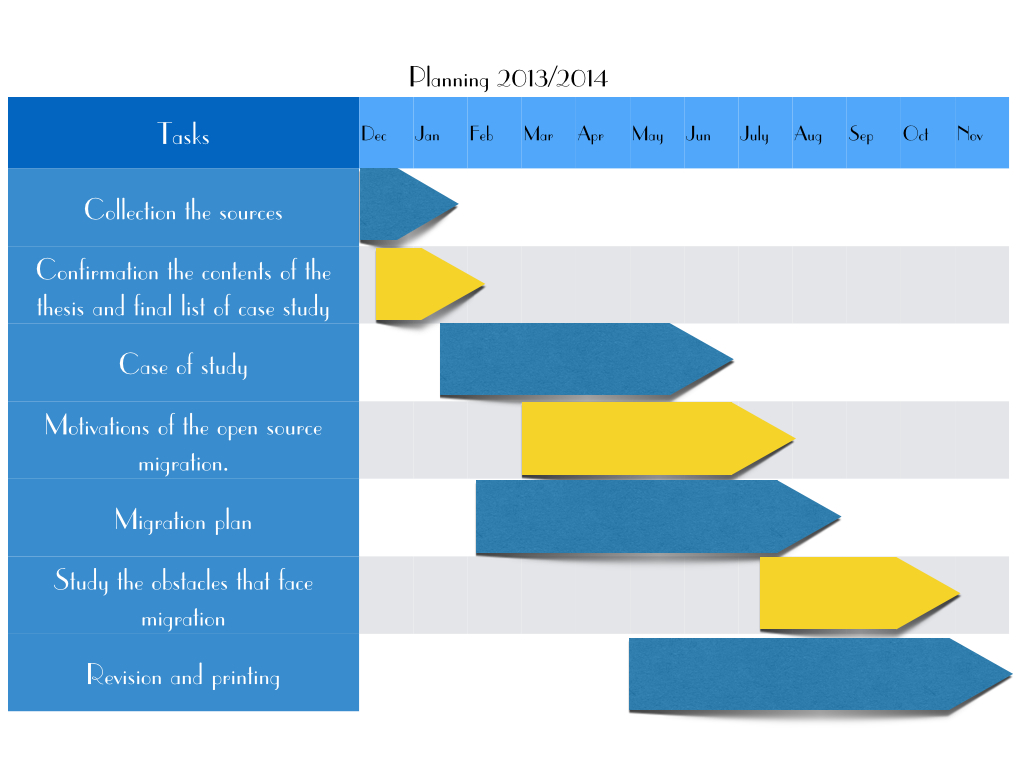
\includegraphics[scale=0.45]{img/planning.jpg}
      \caption{Work Plan and Timeline}
      \label{fig:planning}
    \end{figure}
The reserch period is from December 2013 to November 2014.
    In Figure ~\ref{fig:planning} shows work plan for this thesis.
 
 
 For paraphrase methods . I've used quotes (") and italic font to identify a direct quote. I've cited the original source in the footnote.
 I've used two methods of putting others ideas into my own words by paraphrasing and summarizing. The original source shown in the Bibliography.
 %----------------------------------
\subsection{How this document is organized}
This document is divided into seven chapters. Chapter \ref{chap:introduction} is the introduction. It explore the rationale behind the research and presents the motivation behind the research. Chapter \ref{chap:Goals}  outlines the goals and objectives of the research. Chapter \ref{chap:Motivations} supports the motivation for using free/open source software Chapter \ref{chap:plans} outlines a basic plan for migration to Free and Open Source Software from proprietary software.  Chapter \ref{chap:Obstacles} outlines certain obstacles that may be encountered during the migration process. Chapter \ref{chap:Caseofstudy}  presents several related case studies. Finally, conclusions are drawn in chapter \ref{chap:conclusions} including lessons learned and future work.

 Wherever possible, the first time an abbreviation is used the expanded version will also be included in Appendix \ref{apn:Acronyms}.
 
 %----------------------------------
 \section{Basic Concepts }
In order to facilitate a basic understanding of this work, the following terms are defined, ensuring that the reader will have a clear explanation of the concepts contained herein:
 
 \subsection{Free software}
 \label{sec:freeopen}
Free software, sometimes referred to as Libre software are programs that, by default, include the necessary licensing at no additional charge to the user which allow the user to
 (i) run the program for any of the allowed purposes, (ii) study and modify the program, and (iii) to redistribute copies of either the original or modified program without having to pay any royalties to the software developers. The concept of free software was conceived by Richard Stallman in 1983 with the implementation of the \ac{GNU} Project. The \ac{FSF}  was likewise subsequently created for the purpose of advocating for free software ideals as outlined in the Free Software Definition which states that free software means software that respects the user’s freedom and community. In essence, users have the freedom to run, copy, distribute, study, modify, and improve the software. A program is classified as free software if the program allows users the following four basic freedoms:

 \begin{itemize}
 \item The freedom to run the program, for any (legal) purpose.
 
 \item The freedom to study how the program works, modifying it as desired.
 
 \item The freedom to redistribute copies without recompense to any individual or entity.
 
 \item The freedom to distribute copies of the modified version to others without recompense to any individual or entity.
 \end{itemize}
  \subsection{Open source}
 The open source movement is a worldwide movement consisting of individuals who believe that the best way to produce software that may be described as sophisticated, robust, and (for the most part) free of bugs is to enlist the cooperation of interested, skilled, and altruistic programmers who are willing to work for free. These individuals are inspired by the twin goals of producing high-quality programs and working cooperatively with other similarly minded individuals.
 
 Outline of Key Conditions of OSS Definition \footnote{ By Feller and Fitzgerald in  \url{http://www.brian-fitzgerald.com/wp-content/uploads/2011/07/open-source-icis00.pdf}}"
 
\textit{\begin{itemize}
\item The source code must be available to users.
\item The software must be redistributable.
\item The software must be modifiable and the creation of derivative works must be permitted.
\item The license must not discriminate against any user, group of users, or field of endeavor.
\item The license must apply to all parties to whom the software is distributed.
\item The license cannot restrict aggregations software."
 \end{itemize} }
 
 Thus it can be inferred from the above definitions and meaning that the free/libre and open source software is the new and innovative software developed for the organizations and companies in order to meet the needs and requirements at challenging circumstances. The initiation and adoption of free/libre and open source software in the companies and the organizations came into existence due to the improvement in the \ac{ICT}. The end users has all rights to edit and modify the codes of the software if possess the License.
 
  The term OSS was adopted as an alternative term to “free” software given the fact that the term was not only less confusing, but that it worked to better describe the embodiment of the concept. The terms “\textbf{open source software}” and “\textbf{free software}” are typically used to describe the same programs, with the two terms often being used interchangeably. In fact, there are those who argue that the use of the two different terms, given their similarities, is simply one of a philosophical, rather than practical, difference between the two, and that the difference is primarily a matter of marketing as opposed to the actual substance of the two. Those who prefer to use the term “\textbf{OSS}” typically emphasize the technical advantages of the software that are present, such as the security of the program or the reliability of the program, while those who prefer the term “\textbf{free software}” tend to place their emphasis on the ethical issues addressed through the use of these types of software or the freedom from control of the developers or distributors that these types of programs offer. \footnote{\url{http://www.osepa.eu/site pages/News/ 43/WhyOSS Look at the numbers Wheeler 2007.pdf}}Regardless of perspective, it is important to note that the differences in these categories are extremely small, with almost all free software classified as open source software and almost all open source software as free software. 
 
 Other alternative terminology used to identify these types of programs includes:   \ac{OSS/FS} ,\ac{FOSS} and  \ac{FLOSS} . For the purpose of this thesis, \ac{FLOSS} is used. this term are intended to indicate that the software described has the characteristics that are implicit in both the terms “open source software” and “free software.”
 
  \subsection{Other terms}
  The below terms are all associated with FLOSS in one way or another and some of them will be utilized throughout the course of this thesis. Figure~\ref{fig:categoriesofsoftware} shows the relationship present between these different types of software.
    %--------------------------------------------
 \subsection*{Careware, also known as Charityware} 
Software that is licensed in such a way that it benefits a charity. There are several different types of careware in existence: free careware is completely free software; open source careware is free with the source code being made available to users, as in the case with text editor Vim which is free and OSS and is released under a license that includes some charityware clauses encouraging users who enjoy the software to consider donating to children in Uganda; and commercial careware, wherein the proceeds from the sale of the software are split between the developer and a supported charity. 
  %--------------------------------------------
    \begin{figure}[H]
        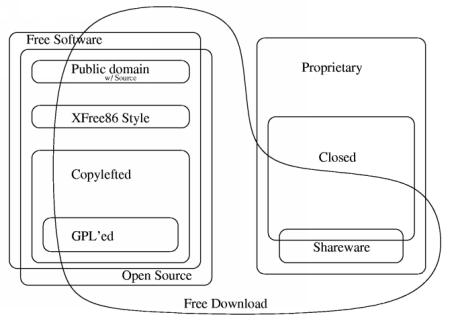
\includegraphics[scale=0.97]{img/free-open.jpg}
      \caption{Different Categories of Software (GNU.org, 2014)}
      \label{fig:categoriesofsoftware}
    \end{figure}
 \subsection*{Copylefted software}
Free software whose distribution terms work to ensure that all copies of all versions carry the same basic distribution terms.
   %--------------------------------------------
    \subsection*{Public domain software}
    Software that is completely free and may be used by any individual for any legal purpose. The software is not copyrighted as it has been donated to the public domain by the holder of copyright and is considered to be a part of the cultural heritage.
  %--------------------------------------------
    \subsection*{proprietary software}
    The opposite of OSS, also known as \ac{CSS}. These types of software are licensed under the exclusive legal right of the copyright holder with the intent that the licensee is given the right to utilize the software only under specific conditions, with the restrictions on the use of the software typically enumerated in the  \ac{EULA}. Restrictions are placed on the use of the software, including the prevention of modification, sharing, studying, redistributing, and reverse engineering. In addition, the source code is not made available for common view.
%--------------------------------------------
  \subsection*{Shareware}
  Software that is provided to users, typically on a limited trial basis that restricts any and all commercial benefits, use, or exploitation of the software. It is distributed without an initial charge, but the user is strongly encouraged to pay a nominal fee for continued use.   
   %--------------------------------------------
  \subsection*{Free software}
A type of proprietary software copyrighted by the developer. The developer retains the rights to control the distribution, modification, and duration of time that the software is offered for use free of monetary charges. This software is typically distributed without its source code, making it differ from free software. 
   %-------------------------------------------- 
   \subsection*{System migration}   
The act of physically transferring data and programs from an old system to a new system. This action is typically accomplished when the old hardware is no longer capable of meeting the needs of the user or when components have become damaged. This process may be simplified by the use of tools and software that allow for the automatic conversion of data up to and including the conversion of the code from one platform to another. 
 %----------------------------------------------------------------------------------------------
   \subsection*{Data migration}
   The process of transporting data between computers, storage devices, or from one format to another; an essential part of any system implementation, upgrade, or consolidation. During this process, software programs or scripts are utilized to map system data for automated migration. Ideally, data should be preserved when completing server or storage equipment replacements, when upgrading, consolidating websites, completing server maintenance, relocating between data centers, or when switching between application versions. Typically, this process requires converting the data into a suitable format for the new system, and it may become necessary to write a program that will automatically process the files being migrated from the old database, automatically inputting them in the new database, especially if the two are organized differently. 
   %----------------------------------------------------------------------------------------------

%-----------------------------------------------------------------------------------
      \newpage
      \begin{savequote}[108mm]
       " Set your goals high, and don't stop till you get there."
        \qauthor{ Bo Jackson}
      \end{savequote}
      \chapter{Goals and Objectives}
      \vspace{-3cm}
      \label{chap:Goals}
 %-----------------------------------------------------------------------------------------

\section{Goals} 

The primary goal of this research is to explore the FLOSS migration in government and private organizations. It is to gain as much knowledge as possible about the migration process so that the concepts learned by this study can be taken home and put into place. By examining the lessons learned by others, it is possible to avoid some of the pitfalls and to make the transition process as smooth as possible.          
                                                                                        
\section{Objectives}
Objectives allow the researcher to turn their concepts and ideals into a working plan. In order to achieve the goals that this research intends to accomplish, the following objectives will be met by this research. 
\begin{itemize}
\item Discover the main reasons why individuals, organizations, and companies are attracted to FLOSS. 
\item Examine the technical, economic, and social benefits of FLOSS.
\item Determine the best method for migration and implementation of FLOSS.
\item Develop a plan for successful migration to FLOSS that addresses the main areas of concern. Provide the main steps necessary for a successful migration.
\item Determine  the main obstacles that organizations face in the migration process.
\item Explore case studies that may provide clues as to the obstacles that the company will face and to explore some possible solutions through examining the experiences of others. and examine the total cost of migration in some cases.
\end{itemize}

\newpage
\begin{savequote}[108mm]
``In real open source, you have the right to control your own destiny.''
  \qauthor{Linus Torvalds}
\end{savequote}
\chapter{Motivations for using FLOSS}
\label{chap:Motivations}
\vspace{-2cm}

%-------------------
    \begin{wrapfigure}[14]{r}{0.38\textwidth}

     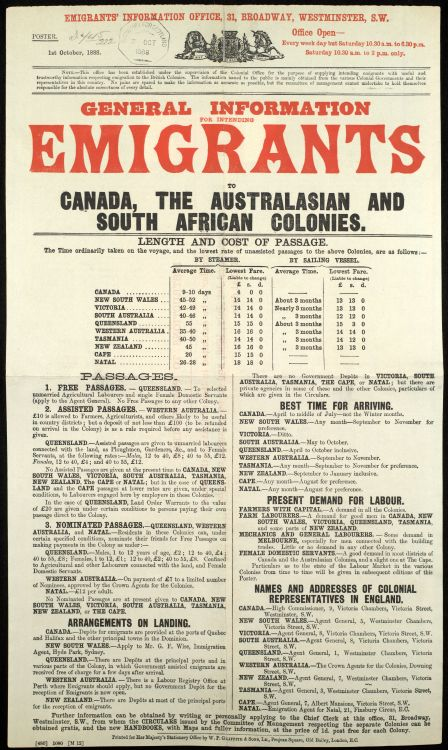
\includegraphics[scale=1.8]{img/Canadaemigration.png}
   \caption  [A Poster advertising emigration to the colonies in 1830]{ {A Poster advertising emigration to the colonies in 1830 \protect\footnotemark} } 
   \end{wrapfigure} 
 \footnotetext{source: \url{http://www.educationscotland.gov.uk/marksonthelandscape/curriculum/citizenship/migration.asp}} 
 
 It is human nature to want to seek out and to improve the manner in which we live, as is evidenced throughout human history. Humans have constantly emigrated from one country or region to another, seeking a better way of life or a better environment. The different motivations behind these emigrations include better employment opportunities, freedom, political or religious rights, famine, drought, disease, poverty, expulsion by armed force, coercion, natural disasters, better educational opportunities, or even better medical facilities.  In today’s day and age, humans attempt to improve their lives in ways other than simply moving in hope of a better life, looking to the use of additional or alternative technologies as a primary example.
 
\newpage

 In this chapter, the motivations of individuals, organizations, and companies involved in the migration to the use of FLOSS will be reviewed, including, but not limited to: public collaboration, reliability, auditability, cost, security, stability, support and accountability, and flexibility and freedom (independence). The benefits of FLOSS, when compared with CSS, are far greater than they originally appear, and while cost is one of the primary motivating factors, the concept of features versus quality and the associated ease of maintenance are other major considerations. Studies have shown that many web servers have attempted to compete with and overcome the benefits of Apache, but were ultimately considered failures as a result of the tactics that were utilized on those other web servers. In fact, there is a particular network practice that allows web servers and browsers to compete in terms of which has the better features or best quality as opposed to just the different tactics; benefits are classified into three types: technical benefits, social benefits, and economic benefits.

 Figure~\ref{fig:Motivations}  shows a diagram of some of the motivation for using the FLOSS.

  \begin{figure}
  \centering
      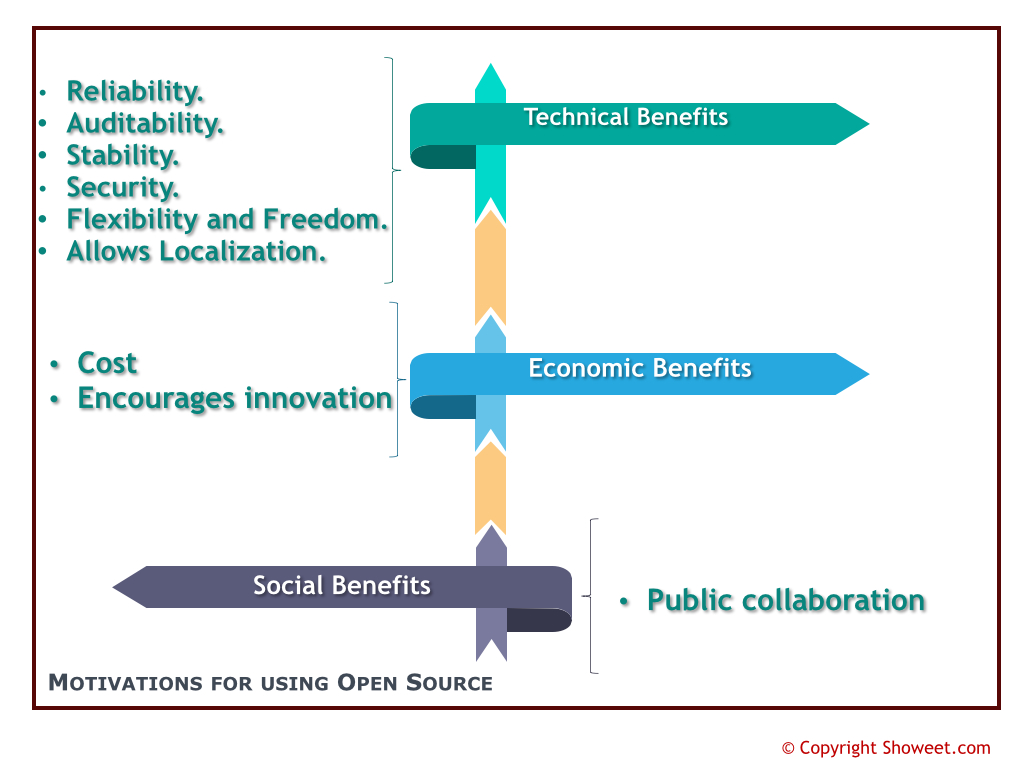
\includegraphics[scale=0.6,angle=90]{img/motivation.png}
    \caption{Motivations for using FLOSS)}
    \label{fig:Motivations}
  \end{figure}

 \section{Technical benefits}

 Technical benefits refer to the reliability, auditability, security, stability, allowance of localization, flexibility, freedom, support, and accountability of a given software, all of which play a vital role in the decision to migrate to FLOSS.


 \subsection {Reliability}
 \textit{``The general business case for open-source is reliability. Open-source software is peer- reviewed software; it is more reliable than closed, proprietary software. Mature open-source code is as reliable as software ever gets.''}
  Eric Raymond\footnote{\url{http://bat8.inria.fr/~lang/hotlist/free/licence/raymond/open-economics.html}}.

 According to Standard Glossary of Software Engineering Terminology\footnote{ \url {http://dis.unal.edu.co/~icasta/ggs/Documentos/Normas/610-12-1990.pdf}} software reliability is defined as \textit{``The ability of a system or component to perform its required functions under stated conditions for a specified period of time''.}

 This mean Reliability refers to whether or not the developed software is free of defects relating to data error and/or loss, incorrect operations, or sudden failures. In utilizing FLOSS, many defects that do end up being found are able to be fixed within mere hours of detection, and the maintenance and update processes are quite simple for individuals and software developers alike. FLOSS has an overall value robustness given the fact that it is embedded with reliable standards, ensuring that not only is the product able to hit the market in its earliest stages, but is highly robust when this occurs. FLOSS promotes quality and reliability through the support of the rapid evolution of the source code and independent peer reviews, two aspects that are missing when dealing with CSS.


 \subsection{Security }
 Since the source code in FLOSS is open, defects and security flaws are more easily found.	Security may seem to be an advantage and a disadvantage at the same time. FLOSS allows its users to access the source code, editing, modifying, and changing the code, which results in potential vulnerabilities, yet it allows all those with access to the code to search and correct those vulnerabilities, quickly and easily rectifying those issues. The transparency offered by FLOSS becomes its greatest asset in this case; while no software is ever fully secure, the amount of transparency offered by FLOSS ensures that it is more secure than other options. It was found that issues were found and corrected quicker in FLOSS than they were in any CSS options. It was revealed that FLOSS had a lower defect density than that of CSS.
 	According to Evans Data Corporation Survey\footnote{Spring 2002 Linux Developer Survey. Wheeler,  David A. Available at \url{http://www.osepa.eu/site\_pages/News/43/WhyOSS\_Look\_at \_the\_numbers\_Wheeler\_2007.pdf}} reports that Linux systems are relatively immune from attacks as security breaches are rare in Linux Environment. 78\% of the respondents to the GNU/Linux developers’ survey have never experienced an unwanted intrusion and 94\% have operated virus-free. The survey shows that GNU/Linux ``doesn’t get broken into very often and is even less frequently targeted by viruses.''
 	
 	These qualities are the reason for the appearance of open source products in response to security requirements. For example, \ac{NSA} in United states released a Linux kernel security module known as \ac{SELinux} which provides the mechanism for supporting access control security policies, including the Department of Defense.
   \subsection {Auditability}
   
   Is a factor at the time the source code gets published. Cross verification of the code with  CSS indicates that FLOSS is far better than CSS as the CSS forces the end user to trust that the vendor and/or developer has worked to ensure that there are no backdoors, that the program is secure, and that there is a flexibility for future modification of the program and adherence to basic security standards. If the developers will not fix the problem, the user has the option of fixing it or hiring someone else to fix it. 
   
   As the source code is not available for CSS, this type of trust cannot be verified by an independent source, with CSS options that this trust is not always founded. FLOSS offers increased levels of confidence on the part of the end user that such issues do not exist by offering this increased accountability.
 \begin{figure}[H]
 	\centering
 	   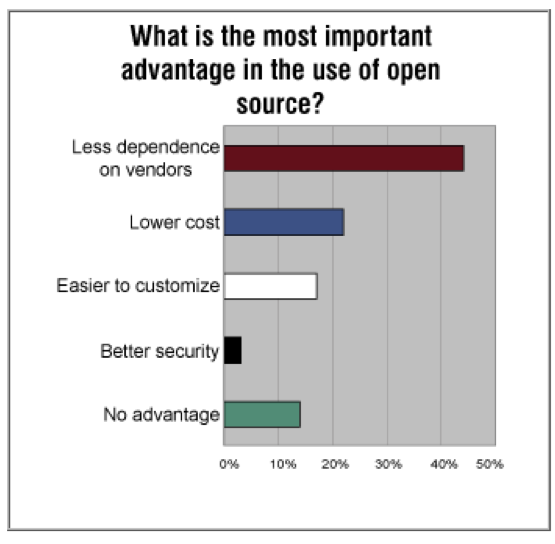
\includegraphics[width=0.6\textwidth]{img/OSSadv.png}
 	  \caption[Advantages of FLOSS]{Advantages of FLOSS (Computer Economics, Inc., 2005)\protect \footnotemark }  
 	  \label{fig:OSSsdv}
 	 	\end{figure}
 	\footnotetext{Source: \url{http://www.computereconomics.com/article.cfm?id=1043} \label{adv}}
 
Figure~\ref{fig:OSSsdv} shows the results of a survey  by ``Computer Economics'' about the advantages in the use of FLOSS, \textit{``The survey indicates that IT decision makers value (reduced dependence on software vendors) as the most important advantage of open source.  This indicates that software buyers must feel some level of dependence on proprietary software vendors, from which they desire freedom.  Such dependence includes reliance on the vendor for maintenance and support and the necessity for the buyer to accept version upgrades that the buyer may not need or want.''}\footnote{Look at previous footnote \ref{adv}} and it also indicating how heavily cost plays a factor in preference.

 \subsection {Flexibility and Freedom } 
  The primary benefit of FLOSS adaptation is the variation that is offered. The flexibility and freedom offered by the implementation of FLOSS by a user or organization is that it facilitates changes, customization, experimentation, and offers freedom of choice to the individual or entity. When implementing CSS, users have to install set applications and files associated with that software, while the installation of FLOSS offers end users with a reliable flexibility of infrastructure, allowing the user to select the applications that they wish to install and utilize out of existing open source options. CSS has a lock in feature that requires the user to input access keys, typically paid for by the user, in order to be able to gain access to certain applications, while in FLOSS all users are able to access all applications, providing further flexibility through freedom. 

  With proprietary software the user is completely dependent on the developer. The developer may be a programmer, but may not have the necessary intimate knowledge of the field to create the best software design for the business. They are in the business of developing software, and may not be as familiar with the needs of the end user as in-house developers. FLOSS allows the company to begin with their needs and then custom design a system that is suited or it, rather than picking something of the shelf that is close, but not an exact fit. 

  \subsection {Stability} 

  Other factors that make users more likely to switch over to FLOSS include the concept of a standard format and increased stability. In utilizing FLOSS, the likelihood of documentation of the different formats is high, whereas in CSS  this is not always an option. The adaptation of FLOSS is more likely by end users as a result, because not only they are able to obtain an application that may be modified and potentially has been modified to meet their needs, as opposed to one that cannot be modified, but that there will likewise be documentation available regarding those modifications. 

  FLOSS allow the user to ensure that the stored data remains readable in the long term, as when using a proprietary format there is the issue that once the format becomes obsolete, the data is, in effect, lost. As many public entities are required to maintain data for decades, the use of FLOSS offers a significant advantage.

  While software vendors and developers are able to discover new ways to retain their customers or end Auditability users, the decision to migrate from one operating system or program to another still resides in the hands of the end user. The primary issue with this is that the average software user does not see this as a choice open to them, believing they have little control over the process and potentially feeling isolated and out of their league, finding this too technical for them, resulting in potential issues for themselves and their business.
 
  \subsection{Allows Localization }
   Localization occurs when the software adapts to the local language for the coding and implementation processes. Source code is often presented in the developer’s primary language; for instance if the developer is from Spain, the source code is likely to be in Spanish, and if they are from China, it is likely to be in Chinese. For other types of software this could cause an issue in problem resolution if the individual attempting to resolve the problem does not speak the primary language, however in FLOSS, there is an option for clients and end users to adapt to their localization, allowing them to obtain the source code in their primary language, allowing users to choose and modify language according to their preferences, a concept quite popular in areas where English is not the primary language.

  \textbf{The Importance of Localization:}\footnote{According to the study ``Free/Open Source Software: Localization'': \url{http://akgul.bilkent.edu.tr/iosn/foss-l10n.pdf}}
 \textit{\begin{itemize}
 \item 	Reduced reliance on imports.
 \item	Local programmers gain expertise and experience.
 \item	Local control over software appearance and functionality.
 \item  New local technical standards and educational opportunities.
 \item Establishment of a local software industry. It is difficult for foreigners to do localization as they do not normally have an intuitive feel for the local language and therefore the language is compromised in most cases.
 \item National policy on local content would not be dependent on the availability of proprietary software or hardware. 
 \item Localization of applications can be prioritized according to the national needs.
 \item Significantly reduces the amount of training necessary to empower end-users to use a computer system.
 \item Facilitates the decentralization of data at provincial and district levels. The same applies to utility companies (electricity, water, telephone), who will develop local language databases, thereby reducing costs and giving better service to citizens.
 \item Helps universities train more software engineers.
 \end{itemize}}
%------------------------------------------------------------------
  \section{Economic Benefits}
  Economic benefits consist of cost and innovation that occur when users are motivated to adopt FLOSS in their organizations or companies. The developers focus on the needs and requirements to be added to existing technologies and amend the source codes in FLOSS, enhancing the features with reliable innovations often free of cost. 
  
  \subsection {Cost}
  
  Cost is considered as a major benefit in FLOSS, especially in comparison to the costs associated with the use of CSS. Software developers collect certain fees under the guise of maintenance, updates, debugging, and so on, causing the costs of CSS to balloon beyond the original price point. While many users do not factor these into the cost of utilizing CSS, companies and organization must pay attention to these \ac{TCO}, making them more likely to see the implementation of FLOSS as a reasonable and cost efficient option. FLOSS offers a potential purchase price of zero, reduces administrative overheads, decreases the amount of accounting that needs to be done, reduces investment needed, reduces licensing fees, reduces upgrade costs, virus protection costs nothing, there is zero vulnerability in downtime and data loss, decreased chances of security breaches, decreased chance of system hacks, decreased chance of attacks, all of which, if occurring, would raise the overall system cost and administrative load. 
  
  Migration to FLOSS also eliminates corporate control of the entity. This is a key reason cited for conversion to FLOSS, particularly for government entities. Migrating to FLOSS
 not only reduces the initial costs of the software, it also reduces the \ac{TCO}. There is no initial cost of the software. There is lower administrative overhead and no need to account for the number of copies that are distributed. CSS usually only allows a certain number of issues of the software before an additional fee will occur.  
  \begin{figure}[H]
     \begin{center}
        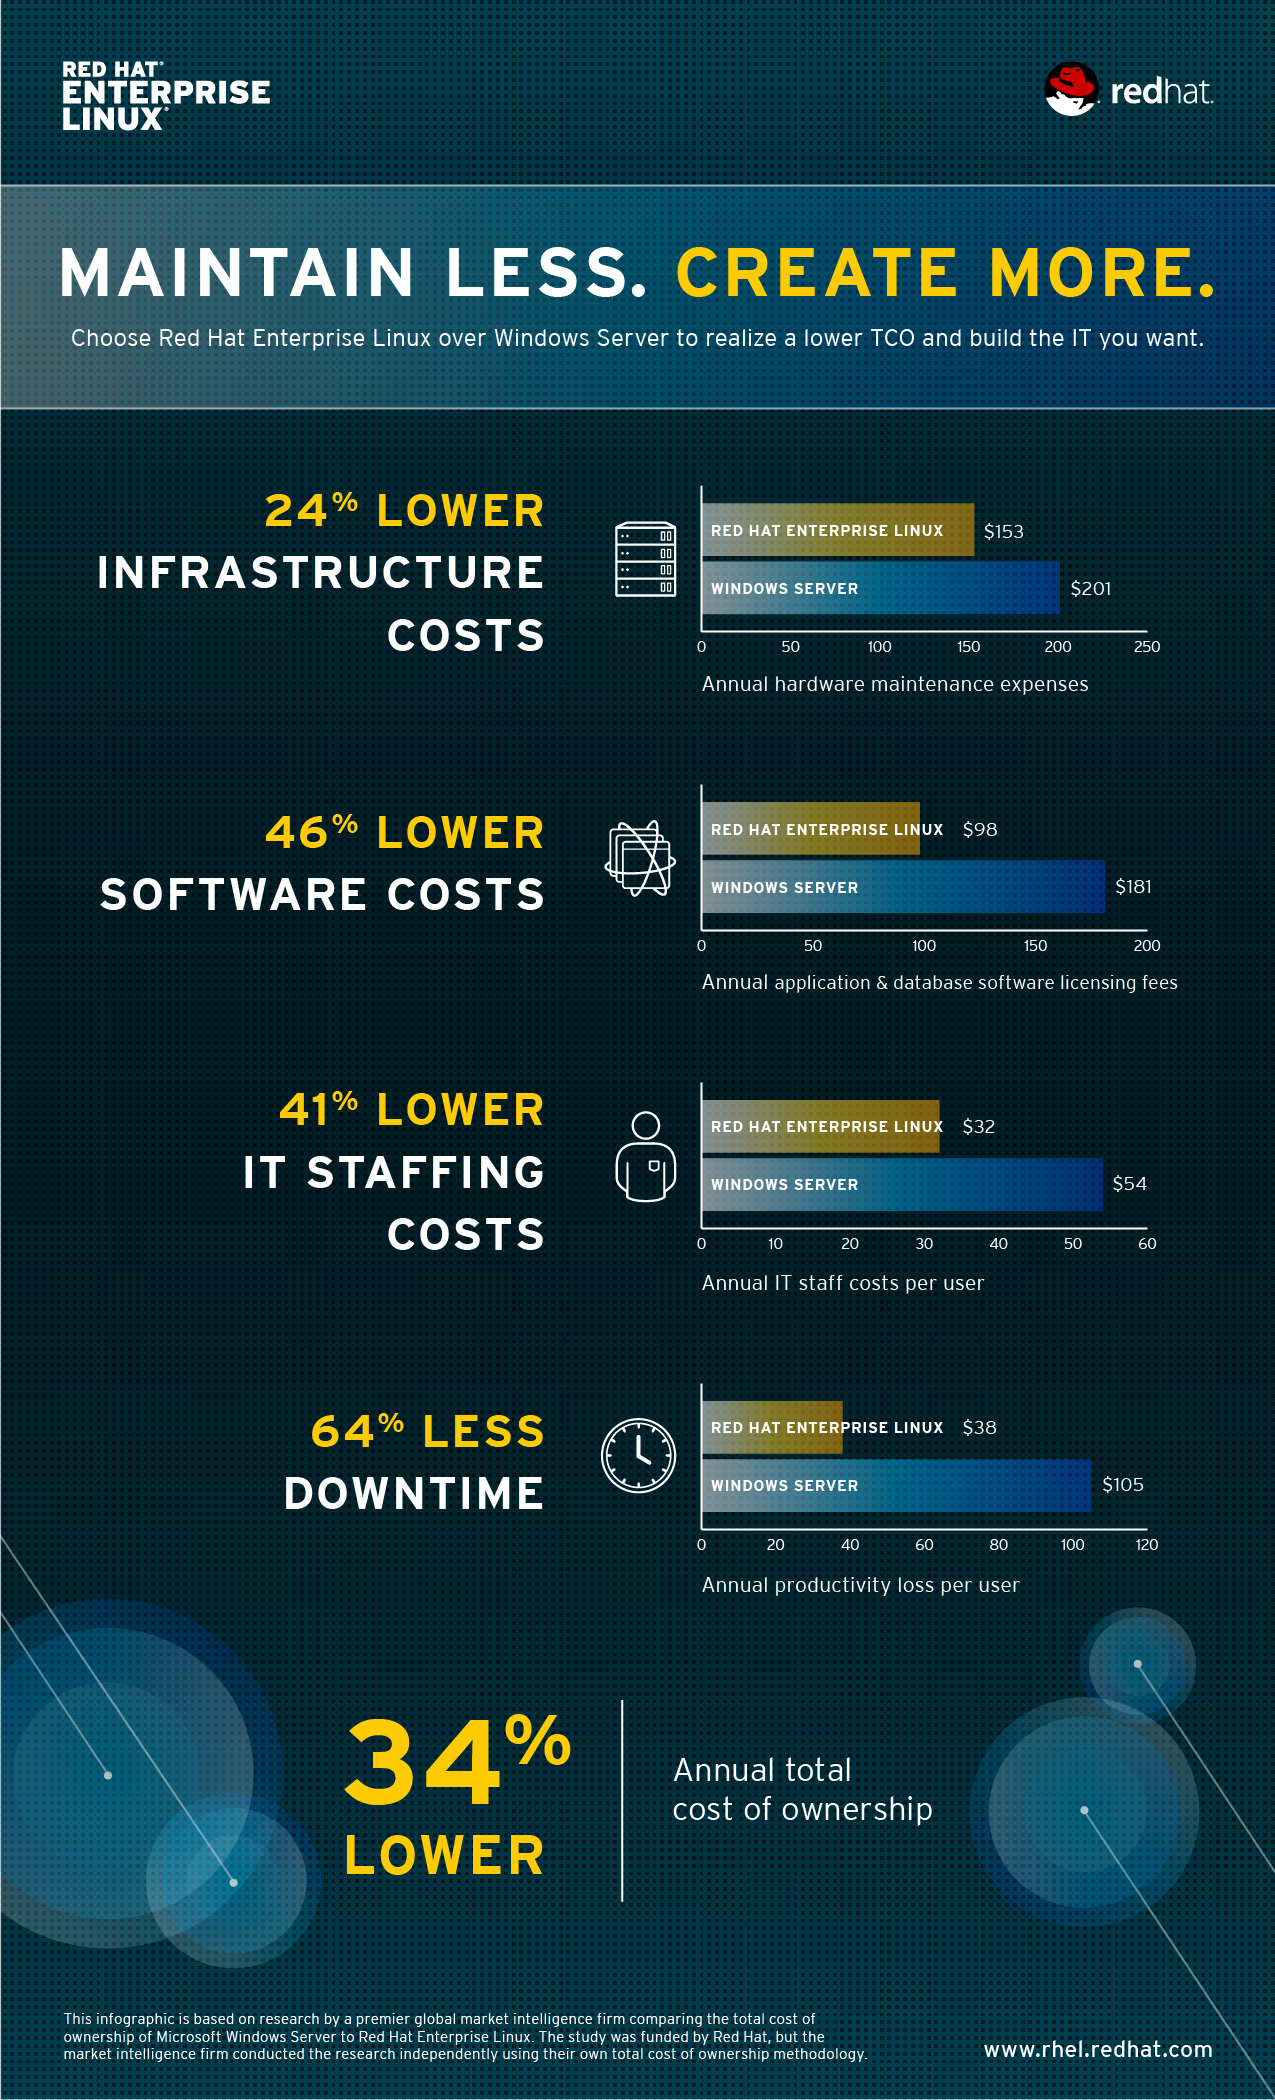
\includegraphics[scale=0.4]{img/RHELFancy.png}
       \caption[Red Hat realize lower TCO] {Red Hat Enterprise choose Linux over Windows server to realize lower TCO \protect\footnotemark}
       \label{fig:RedHat}
     \end{center}
       \end{figure}
  \footnotetext{Source:\url{http://www.redhat.com/en/about/blog/how-red-hat-enterprise-linux-trims-total-cost-of-ownership-in-comparison-to-windows-server}\label{fo:redhat}}
 In a study by Red Hat, compared costs and efficiencies of two commonly deployed IT infrastructure platforms: Red Hat Enterprise Linux and Microsoft Windows Server.\textit{``Based on expenses measured per year per user, the study recorded significant annual savings for Red Hat Enterprise Linux versus Windows in three cost categories: server infrastructure costs (29\% lower), IT staffing costs (41\% lower), and costs from lost user productivity (64\% lower). Taken together, Red Hat Enterprise Linux systems provided an annual TCO savings of 34\% over Microsoft Windows.''}\footnote{look at previous footnote  (\ref{fo:redhat})}

 
Figure~\ref{fig:RedHat} shows how infrastructure platforms based on Red Hat Enterprise Linux experienced the TCO  to 34\% lower annual TCO per user compared to systems running Windows Server.

 \subsection{Encourages innovation}
  The use of FLOSS offers an increased chance of innovation, which increases the overall value of the software itself. In the combination of cost, reliability, and innovation, FLOSS ends up outperforming CSS  each time.
  The innovations in the technology have impacted the FLOSS users to generate plans and motivate the FLOSS developers to enhance the current technology with up-gradation. The innovative technologies in the ICT development around the world have attracted several users to adopt the FLOSS instead of staying with the CSS. For instance, in the study conducted by Zhussupova and Rahman\footnote{Zhussupova, A. and Rahman, A.A., (2011), ``Open Source Software Adoption in Public Organizations of Kazakhstan'', Journal of IEEE: Conference on Open Systems, 7(1), 417-502, 2012, Elsevier.} the organizations in Kazakhstan and Malaysia, shifted from their traditional licensed based technologies and adopted the FLOSS in order to get better results. Other studies that have proved the intense use of FLOSS in biometrics and aeronautics and space have also proved that the results attained by the researches in their study with the help of FLOSS was reliable than that of the results that were attained with the help of CSS. The innovative technologies in the field of education adapted themselves to the FLOSS platforms where the staffs at the universities and the libraries can utilize the exploratory design of the software where the training is unnecessary and the support of the communities was approachable. Since there are no particular ways to seek support directly from the software developer in order to clarify the doubts in the FLOSS products, the users encouraged the developers to come up with innovative technologies where they can seek help from other developers or users in the community or the developer himself would provide solutions by creating his own community, thus both the users and the developers would be benefited. Allowing for all to adjust the software, as their imagination lets them.  
  
  \section{Social Benefits }
  The social structure that is created by FLOSS encourages programmers to become users, and vice-versa, as this allows the users and the programmers alike to understand the needs of the other. The most natural relationship that occurs is one that is directly reciprocal between the two. Programmers write the software for the users, and the users suggest features to programmers and report bugs when they are found, allowing for a closer and more mutually beneficial relationship between the two.
  
  While the social and societal value of FLOSS is not always highlighted by either the public or the private sector, it results in the unfettered sharing of knowledge, increases the formulation of rules, and works to redefine methods of data manipulation and procedures. Knowledge works to ensure that a better future may be shaped from the current state of economics and as a result of the productivity of the situation. Opinion leaders and experts often advocate to their customers that knowledge should be equally shared and spread around the globe and within society as freely and widely as possible.
  
  \subsection{Public collaboration}
  Public collaboration is one of the major factor that benefits the organizations and the businesses with the FLOSS implementation. Behind each and every projects, several programmers focus specially on collaborating to generate and improve a flawless website with better framework. Though there are several companies that makes use of proprietary or workstations or home built systems as their website frameworks which were created by themselves, there are companies that make use of the FLOSS like Drupal and WordPress which were developed through the talents of thousands of developers. Thus the public would be motivated by the FLOSS preferred by the companies rather than using the CSS.
  \newpage
  
  It may be inferred from the above identified benefits that FLOSS is: cost free, license fee free, user friendly, reliable, auditable, a public collaborative, securable, stable, supportable, accountable, flexible, and independent, enable localization of software to native languages, faster technology development through collaborative innovation and development of the domestic IT industry, generate opportunities in the form of more and better jobs, by learning and training more personal growth opportunities. better businesses, better government by more efficient institutions, and reduction of dependence on monopolistic CSS vendors.
  
  The FLOSS being zero cost provides faster ways in adapting to the technologies in organization than that of the proprietary software and also provides the companies with license free models such as service based models deviating from the traditional models. The adoption of FLOSS is quite easier and faster and the software provides the end users with ease of access and synchronization.
  
  As a result using FLOSS is a reasonable or even better compared to CSS. This result is also supported by studies by various research, but benefits offered depend largely on context, with the benefits remaining higher when compared with CSS. The key factors that makes FLOSS more reliable are that developers are usually also users of the software, developers are members of a community of developers, public availability of the source code and fast bug removal practices since thousands of independent programmers testing and fixing bugs of the software.

\newpage
\begin{savequote}[108mm]
 ``Plan your work for today and every day, then work your plan.''
  \qauthor{Margaret Thatcher}
\end{savequote}
\chapter{Migration plan }
\label{chap:plans}
\vspace{-2cm}
%--------------------------------------------------------------------------------------
 
 Any successful migration must have a plan that approaches the process in phases that take the proper concerns into consideration at the proper time. This chapter  proposes a three phase process. The first phase is the planning process. The second phase is the actual migration. The third phase is implementation and testing. A majority of the work should be placed in the planning stage. An effort should be made to identify and devise solutions for any obstacles or challenges that should arise. The following outlines the phases of the migration process as shown in the Figure~\ref{fig:migrationplan}. 
 
\section{First Phase:Pre-migration}
 
 The pre-migration process is the most critical to the success of the project. In this phase, the goals and vision for the migration will form the guiding processes for the rest of the migration process. The needs of the organization must be the primary concern in the design and implementation of the new system. It is critical to have measurable goals and objectives. The organization must know where it is going before it can design a means to get there. The needs and goals of the business is the first, and perhaps most important phase of the process.                                                                                                                                

 \begin{figure}[H]
 \centering
    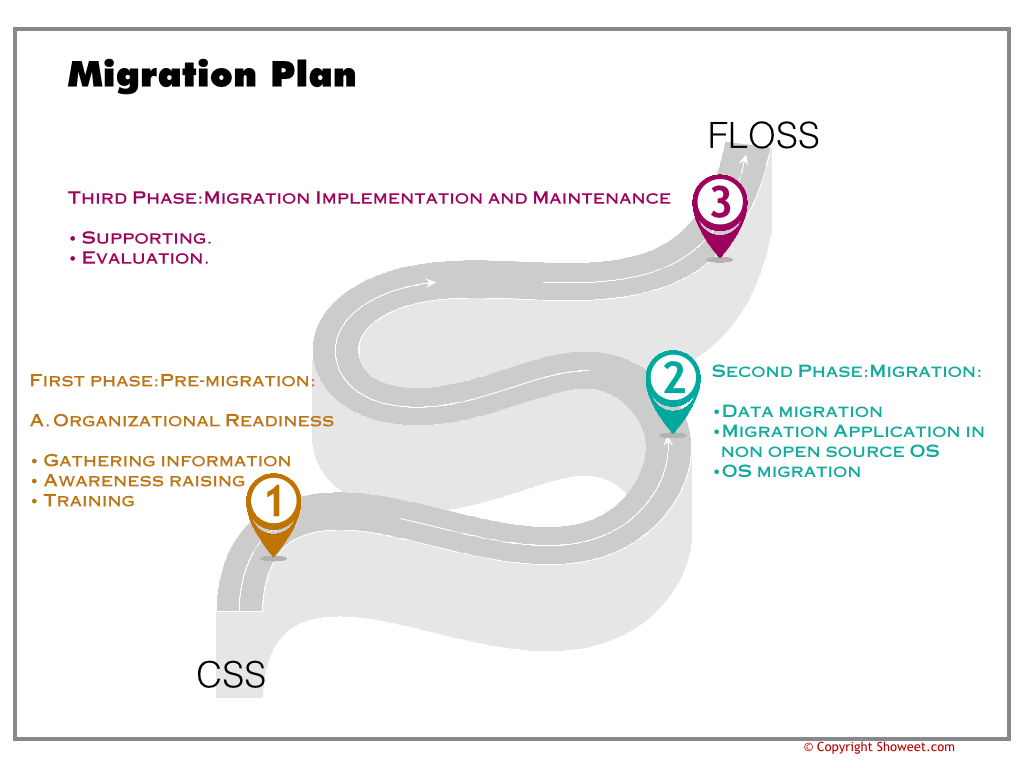
\includegraphics[scale=0.6,angle=90]{img/migrationplan.png}
      \caption{Migration plan}
      \label{fig:migrationplan}
    \end{figure}
    
    \subsection{Organizational Readiness}
    
    Once the company has clear goals and knows what it needs the project to accomplish, it can then set about the task of assessing the readiness of the organization for the transition.
    
    \subsubsection{Gathering information}
    The first step in assessing organizational readiness is gathering information. 
    This must include a thorough audit to gather as much information as possible on existing hardware, software, and the needs that these component serve. The electrical and mechanical components of the building may have to be modified to accommodate the new system. All of these needs must be taken into consideration when assessing the readiness of the organization during the information gathering stage.
    
    Another component of readiness is personnel. An assessment needs to be made or current staff and any future staffing needs that will result from the migration to FLOSS. The organization needs to ask the question of whether they will need to hire any additional technical support, consultants, or training personnel in conjunction with the change. They need to assess whether these needs will be temporary or permanent changes to the organization. The organization also needs to determine if the current staff is prepared for the change and what needs to be done to get them ready. 
    
    There are many sources of information that should be considered. It is important to gather and compare as much information as possible from as many sources as possible. Personal interviews with various department executives to determine their needs is one source of information. The people that will be working directly with the new system will be the best sources of information within the organization.  In addition to sources of information within the organization, outside sources of information may be valuable as well. One can also examine case studies of similar migration projects. For instance, one might talk to others who have undergone similar changes in their organization. They can provide valuable insight as to any unforeseen challenges that one may face. One needs to gather information on the type of data that the organization utilizes and how it is organized within the current business system.  This information can be found by consulting with employees who produce the data and their managers.
    
    \subsubsection{Awareness raising and building a FLOSS community}
    
    \textit{ "Many people focus on encouraging more users to switch to free software. That's a useful thing to do. But that alone is not enough to bring us to freedoms that endure. If we gave everybody in the World free software today, but we failed to teach them about the four freedoms, then five years from now, would they still have free software?"}\footnote{Richard Stallman  presentation \url{http://blogs.fsfe.org/ciaran/?p=57}}
    
    Raising awareness in the organization goes beyond simple knowledge that the change will take place. Raising awareness includes getting people excited about the change and raising the level of support within the organization. It is about gaining managerial support and support on all levels of the organization. People must be made aware of the importance and advantages of the change for the organization. This support will be valuable if any challenges should arise during the process. 
    
    In addition to raising awareness within the organization, there also needs to be some consideration of community awareness too. Before involvement on the migration the community must have a clear understanding of the reasons to migrate.
    Building a FLOSS community, and participatory contributing are essential and recurring activities that enable FLOSS projects to persist. 

    The community will interact with the system, either directly or through organizational representatives. When public funds will be used, the public needs to be informed of the reasoning for the change and what they will mean for the community. Community awareness can be raised through public workshops, formal classes in schools, and town meetings. The mass media can also be used to raise public awareness through newspaper articles and stories by local television stories on the benefits of the new FLOSS. 
    
    \subsubsection{Training}
    The final consideration of the first phase concerns training. Prior to beginning implementation of the software, people must be trained on how to use it. In some cases, a majority of the changes will be on the back end of the system. The average user will not notice significant differences. In other cases, the migration will mean learning an entirely new of doing business. Without sufficient training, employees will be likely to have problems. This will lead to a dislike and lack of support for the new system. Proper training can help to eliminate these issues. 
    
    Training will include classroom training at the facility normally used by the organization for those purposes. and also can be by creating an e-learning environment. Training will include a variety of materials that cover the reason for the change, how the change will benefit the company, and how to operate the new system. It will give them hands on experience and will allow them time to ask any questions that they may have. Most importantly, it will provide them with information on where they can get help once the system is up and running.
    
    \section{Second Phase: Migration}
    
    The second phase of the migration process is moving the data and records from the old closed software to the new open platform. If compatibility issues exist, this is where many problems will occur.  A step by step and start with non critical systems; process needs to be devised that allows for as little disruption of the daily business routines of the organization as possible. This process will be different for every organization and for every migration. A plan for backing up date prior to migration is essential in case unforeseen circumstances should arise. The phases of the migration will cover four different areas. 
    
    \subsection{Data migration}
    
    Data migration to the new system is the most critical phase of the migration process. A data back-up plan is essential to prevent data loss. The ease or success of this phase of the plan depends on the compatibility and similarity of the two systems. If a large amount of data is involved, it may be possible to try a small-scale trial migration before attempting the large scale migration process. 
  
    It is important to divide the data into three categories:
    \begin{enumerate}[itemsep=0ex]
    \item Data which can be get rid of.
     \item Data which must be kept it is useful and in open format such as PDF or Postscript, or can be easily translated into open format.
      \item  Data which must be kept but which is in a closed format which cannot be easily translated into an open one. This data may need copies of the CSS. The cost of these applications will need to be estimate.
    \end{enumerate}

    Data migration will entail moving the most critical data first. The application migration will take place in stages. First the lightweight, smaller applications will be migrated. Only the data that accompanies these small applications will be transferred first. Next, application and operating systems will be transferred. The data necessary at each of these junctures will be transferred at an appropriate time. The data migration process will be dependent on the timing and scheduling of the migration of the applications. 
    
    
    \subsection {Migration Application in non FLOSS OS}
    
    It is possible to run FLOSS and proprietary software in conjunction with each other, creating a highly customizable option that can fit almost any business need.
    
    The key to the success of this strategy is in the FLOSS. It is often prohibited to modify the proprietary software, but the FLOSS allows the developer to work around this obstacle without modifying the proprietary software. 
    
    The case study of the migration from closed to FLOSS in Zaragoza, Spain,   mention in detail later\footnote{Go to Section~\ref{Zaragoza}} provides a plan for migrating applications with as little interruption of business operations as possible. Following this example as a lead, applications must be prioritizes and moved according to their size.  The first applications to be migrated were lightweight  applications such as replacement of the Internet browser to one that is compatible with FLOSS. Next they replaced Outlook with Mozilla Thunderbird. They replaced their FTP client to one that was compatible with FLOSS. They also replaced Windows Media Player with VLC, a program that is more compatible with FLOSS. 
    
     Making these small changes first allowed people to be able to get used to the new system in a way that broke them in slowly. After the lighter weigh programs had been moved to FLOSS, they then moved the main office applications. During this phase, they would be using the new FLOSS system of all of their work. Moving the office applications is the phase that will have the greatest impact on the experiences of the employee. However, because they are familiar with the new system from the migration of lightweight applications, it is expected to make transition of the office system easier. This staged approach will yield and easier transition for the employees who will use the new FLOSS system.          
  
   \subsection{OS migration}
    \label{opensource_OS} 
    The operating system was the last item to be moved.  There are many details that cannot be provided without information on the two operating systems involved. Operating system migration is a specialized field and there are many nuances to the process. It is recommended that a consultant be used for this part of the migration process. There are many choices for operating systems that can support FLOSS.
    
    Linux is the most common operating system for both FLOSS and hybrid systems. Linux is highly configurable, making it the system of choice for many large scale operations. However, this is not the only operating system choice. The most important consideration when choosing a new operating system for a backbone is to consider the current and future needs of the organization. A system that can be easily expanded in the future is the most economical choice. Consultants and outside contractors are the most valuable resource in the operating system migration. 
    
     \section{Third Phase: Migration Implementation and Maintenance}
     \label{Implementation}
     
     The third phase of the migration is final implementation. If you have taken the time and given the proper attention to these previous phases, they may be a time for celebrating the new system. Prior to full implementation, the new system should be tested any bugs addressed. The first few days of weeks may be difficult as everyone learns the new system. Supporting will play a role in getting through this initial phase. 
     \subsection {Supporting}
     
     It is essential to consider having enough support available during all of this phase. These supports can be internal or external to the organization. It may be possible to transition these support personnel to permanent technical support. 
     
     After the migration is complete, a support system will be set up for employees who use the system on a daily basis. This will include a special help line number that they can call to have their questions answered. Telephone support is expected to be one of the main form of support used in a majority of the situations. 	There will also be a support website set up that will have a troubleshooting tool that can walk customers through some of the most common problems that they will encounter. They will also have the option of contacting the support department through email or chat. Employees will have many different avenues to contact support, depending on the urgency of their issue. 
     
     Once this initial learning phase is complete, the organization can then turn its attention to maintenance of the new system and any improvements that it wishes to make in the future. The maintenance that needs to be performed depends on the system that is chosen as the FLOSS platform, the amount of data processed, and other factors. This will be an ongoing process throughout the lifespan of the system. The maintenance plan will be set into a formal written form that outlines all of the procedures and the schedule in which they will be performed. 


 \newpage
 \begin{savequote}[108mm]
``If you expect life to be easy, challenges will seem difficult. If you accept that challenges may occur, life will be easier.''
  \qauthor{Rob Liano}
\end{savequote}
 \chapter{Obstacles that face migration}
 \label{chap:Obstacles}
 \vspace{-2cm}
 Migration is a part of the software life cycle. The concept behind migration is that it should occur as smoothly as possible and without interruption of vital business functions and services.

 Migrating from CSS to FLOSS has its own set of challenge and obstacles. The following will explore some of the challenges and obstacles of migrating to FLOSS. 
 
   \begin{figure}
    \centering
        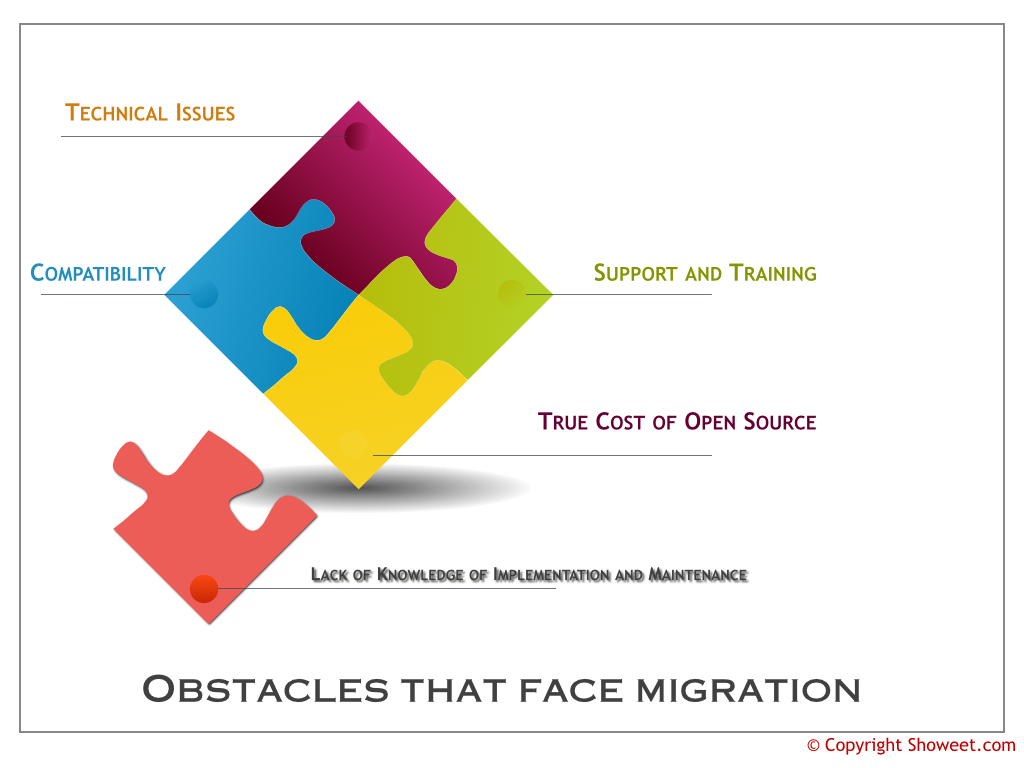
\includegraphics[scale=0.6,angle=90]{img/obsticals.png}
      \caption{Obstacles that face migration}
      \label{fig:Obstacles}
    \end{figure}

 \section{Support and Training}
 \label{sec:Support}


 The migration to FLOSS may be a culture shock to some companies. They will have to get used to resolving problems for themselves, rather than picking up the phone and asking a service representative. However, they also have more freedom to create a software package that is suited to their exact needs. This may be a key advantage for businesses that are in emerging or new areas of business. 

 FLOSS users are often surprised to find the amount of support available from developers and the user community, not to mention how approachable and reasonable the support is. While paid commercial support is ideal for those who need assistance on a regular basis, it is not necessary and is typically only recommended for commercial use. FLOSS ensures that defects are identified and rectified within a timely manner, and as a result of the fact that the software is used by so many, all warranties and liabilities, such as fitness for purpose and merchantability are offered, similar to CSS.  Proprietary vendors typically sell contracts with agreed levels of services, support, or warranties to end users, while FLOSS allows a third party to provide an equal or greater level of support.




 For companies that are used to calling up technical support every time a question or issue arises, the migration to FLOSS may be challenging. Often there is no formal support structure for the system. The advantage is that FLOSS are generally considered easier to administer than CSS. There is usually plenty of information available on open source databases. At worst, the company may have to hire their own expert, which is still cheaper than many CSS licenses. Aside from a lack of support available, there is also no warranty or accountability. This is often and issue with many software migrations. If something goes wrong, the company is on its own. 

 Many companies are choosing to migrate to open source systems such as Linux to free themselves from the increasing financial burdens of Microsoft. A study\footnote{Jashari, Bardhyl and Stojanovski, Filip. Challenges and obstacles: Usage of Free and Open Source Software in local government in Macedonia. Metamorphosis Foundation\label{ftn:Macedonia}} of the migration of government servers Linux  among the governments of local municipalities found that a lack of support was the number one reason why certain municipalities refused to migrate their platforms. This lack of support was a key hindrance to the willingness of municipalities to switch their systems to FLOSS.

 Many companies solved the issue of support by having their own internal team of system administrators and support personnel. Others hired off-site support through hosting and infrastructure partnerships. Some organizations used a combination of these two choices. In larger organizations, there was often a separate division outside of the regular IT department to handle issues with FLOSS migration, programs, and support. The type of system and support set up that worked depended on the size and individual needs of the company.  Even with adding the staff needed to handle maintenance and support functions with the FLOSS, a majority of the companies still reported that the system was a good value for the money.

 \subsection{Training Issues}

 Due to the popularity and familiarity of Windows based systems, many FLOSS platforms have tried to mimic the look and feel of the familiar Windows based systems. However, they are different and the transition can be difficult for some users. Training is needed to overcome many of the user issues associated with the use of the new system. Many municipalities indicated that they would be willing to adopt FLOSS, if training and support were provided. As there is no single entity that accountable for the software, there is no system in place for formal training. Companies that migrate from CSS to FLOSS may need to develop training programs themselves and bear the expense. Having an in-house expert or internal person responsible for support and training may be one solution to overcoming this obstacle.
 
\textit{``There is also another, very human problem to overcome: that most people don't understand computers or software, but have memorized all the keystrokes and mouse-click patterns they need to get through the day, so the second they are given a new program they need to memorize a whole new set.''}\footnote{\url{http://www.largo.com/eGov/apps/document/center.egov?view=item;id=1793}} This can happen any time when new software is introduced in a workplace environment. But train people and answer users' questions will help new users to overcome this difficulties.

 \section{Compatibility}
  Compatibility is an issue in the willingness and success of migration. Government and other large corporate system can have thousands, or even hundreds of thousands of documents and records that they must be able to open on the new system. In the case of moving into Linux, an enterprise has to make sure that whatever software it uses is compatible with the Linux OS.
  The older the version of the CSS, the more prevalent compatibility issues will be. In many cases, the new FLOSS does not only have to be able to open them, they must be able to edit and update them too. These are the key challenges being faced by companies that choose to migrate to FLOSS. 
  A mismatch of programming language and integration is another challenge to the migration to FLOSS. Open source systems can be complex because of the different philosophies and approaches that went into them. Concerns over incompatibility means that the new system may have more bugs than the old one. Being an open source system, these bugs can be corrected by the operators and administrators of the system. However, migrating to a system that has more bugs than the old one is not consistent with the goal of having as few glitches as possible in the migration process. Incompatibility in programming can bring the business to a stop during the migration process. 

  The system is not perfect and not every piece of third party software will run on every system, but it provides many more choices than closed systems.
  Although not all of our favorite programs will run in Linux, the good news is that many of the FLOSS alternatives that have been developed are completely free of charge.


  \section{Technical Issues}
  Aside from compatibility issues linked to the ability to open and edit documents, other technical issues can arise. One of key issues is that proprietary software is often designed to remain proprietary. Reconfiguring the old data can be impossible, because of stop gaps placed in the proprietary software that are intentionally designed to prevent it from being changed. Retooling the old software can be one of the biggest challenges that the company faces. 
  The cost motivation for moving to FLOSS can be compelling, but resolving the technical issues can quickly increase the initial projected costs of the project. Even though technical issues may increase the cost of migration in some cases, it may still be the cheapest route when one take a long term perspective on the cost structure of the project. Using a slower migration approach and breaking the process down into smaller sections can help to mitigate these rising costs. 
	
  \section{Lack of Knowledge of Implementation Procedures and Maintenance}

  A recent study reported that a lack of knowledge of implementation and maintenance issues were one of the reason for failing to migrate to the FLOSS\footnote{Macedonia Survey(Look at Section.\ref{sec:Support}, footnote~\ref{ftn:Macedonia})}. 
  Having a local consultant available to assist with the implementation, maintenance, support, and training issues would make them more willing to complete the migration to FLOSS. These study results may apply to other migrations to FLOSS. This insight may provide solutions in other FLOSS migration circumstances as well.  

  FLOSS takes a team approach to implementation and development. The average user is unfamiliar with the software or possesses the level of expertise necessary to participate in the team environment.
  A lack of oversight in the development of the software is a challenge to the adoption of FLOSS. Uncertainty of the future of the software is another obstacle to the adoption of FLOSS. 

  The lack of a central entity with a unified plan for the future of the development of the software project is a reason for hesitation to migrate.
  There is the possibility that future renditions of the software may not be compatible or useful to the organization.
  Accountability gives managers confidence in the direction of future software upgrades and directions. 
 

 \section{True Cost of FLOSS}
 The ability to have a software package that does not have additional licensing fees and continual costs associated with it may sound enticing, but there are many hidden costs that must be considered before an honest evaluation of the costs of the open source system can be determined. Although FLOSS eliminates many of the additional costs of closed systems, some did not consider them a good value for their money. Some of these reasons were a lack of specific applications, inferior quality, a lack of features, lack of community backing, incomplete implementation, programs that do not work correctly, and complex code bases.
 When the migration is successful, it can save the company money. When interoperability problems, compatibility problems, and system problems plague the new FLOSS, it can end up costing more in the end, negating the savings. If the migration fails completely, then it will cost even more to migrate the system back to the old backbone, representing wasted money and wasted time. Not every migration to FLOSS is successful\footnote{Phipps, S. Triumph and Disaster: Two migrations to Open Office. Open Sources}. Sometimes companies skipped steps and cut costs during the migration in the wrong places. This led to failed migrations and ended up costing the company more in the end. These cases highlight the importance of foreseeing the challenges before the migration and making certain that the migration goes as planned. 
 
 The cost savings and freedom to design as one chooses are key reasons for an upsurge of FLOSS packages. However, a majority of the world is still tied to proprietary software and does not plan to make the switch to FLOSS. 
 

 
 Although this research focuses on the advantages of FLOSS  and promotes it as the preferred solution in many cases, it may not be the solution for everyone, particularly those who are not ready to make the transition. 
 
 FLOSS is often a clone of proprietary software, with enough degrees of difference to satisfy the patent and copyright laws. There is no doubt that there is some functional and well-built open source out on the market today. More is developed on a continual basis. However, FLOSS is still not a replacement for proprietary vendors due to obstacles that it presents. Many versions of FLOSS require a higher level of knowledge than vendor software, making it more challenging than proprietary software. It has been suggested that until more user friendly versions of the software have been developed that FLOSS only be used for back end applications.

 FLOSS faces many challenges that it will need to resolve in order to encourage migration from proprietary systems. 
  The main reasons for this unwillingness to migrate is based on an unwillingness to take on the responsibilities that go along with open source that can be solved by politicians promote and support.
  
  
 
\newpage
\begin{savequote}[108mm]
"Nothing is impossible, the word itself says 'I'm possible"
   \qauthor{Audrey Hepburn}
\end{savequote}
\chapter{Case of study}
\label{chap:Caseofstudy}
\vspace{-2cm}
The rise of FLOSS has caused many organizations and even many governments to consider the possibility of a migration. This chapter will describe some of the successful cases of migration to the use of these types of programs. 
%--------------------------------------------------------------

\section {Zaragoza ,Spain}
\label{Zaragoza}

\begin{figure}[H]
\centering
    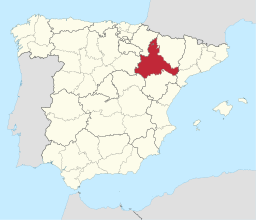
\includegraphics[scale=0.8]{img/Zaragoza.png} 
  \caption{ Zaragoza City}
    \end{figure}

Zaragoza is one of the largest cities in Spain; the city itself boasts approximately 5,000 employees who offer a wide range of services to the approximately 660,000 people who reside therein. 

\subsection{AZLinux}
AZLinux is the Linux distro, based on OpenSUSE, that was created and promoted by the city council of Zaragoza. Since 2003, the promotion and use of  FLOSS by the city has become one of the identifying marks of the Zaragoza City Council, in respect to IT matters.

In 2005, the City Council adopted a motion that urged the city’s local government to promote the use of  FLOSS, especially by all municipal employees. 

\textit{"We have to explain ourselves to users, technicians, public managers and almost every body else. We discovered that fear, uncertainty and doubt are very effective tools to hinder our progress. Fortunately, our politicians promote and support our IT policies to switch to free software. Obtaining and maintaining this political support is crucial to overcome difficulties in the migration process."}\footnote{Eduardo Romero, computer technician at City of Zaragoza in\url{https://joinup.ec.europa.eu/news/es-zaragozas-move-complete-open-source-desktop-going-plan}}

As a result of this motion, considerable savings have been made in regard to the associated licensing costs that were previously being paid out and expert knowledge has been gained, knowledge being shared with the local community. 
\begin{table}[H] \centering

\begin{tabular}{| c| c |}
\hline
PCs with OpenOffice & +3,000\\\hline
PCs using Linux   & +600  \\ \hline
Free Software      & 100\%  \\ \hline
Servers Using Linux  & 80\% \\ \hline
Computer Literacy Centers & 17   \\
\hline
\end{tabular}
\caption{Zaragoza Implementation of Free Software}
\label{table:Zaragoza implementation}
\end{table}
In the same year, an agreement was signed with HispaLinux that setup a building dedicated to the promotion and use of   FLOSS within the city; seven years later, this facility is still running and has since become the focal point for all free knowledge related activities and serves as a tele-center for those that have a need of it.

As Table \ref{table:Zaragoza implementation} indicates, the number of those who are utilizing the Linux computer literacy centers and those who have taken advantage of the switch over to FLOSS is far greater than could have been anticipated. \footnote{\url{http://www.zaragoza.es/contenidos/sectores/tecnologia/Estrategia-Ciencia-Tecnologia-en.pdf}}


\subsection{Migration plan}

  The Zaragoza migration took place in three phases. First lightweight applications were transferred, then office operations, and finally the operating system. This method resulted in the least amount of downtime for the business the results of the study found that this migration method was an effective means to perform the migration. 
 \footnote{\url{http://www.slideshare.net/slides\_eoi/migracin-a-software-libre-del-escritorio-del-ayuntamiento-de-zaragoza}}
 \begin{figure}[H]
 \centering
     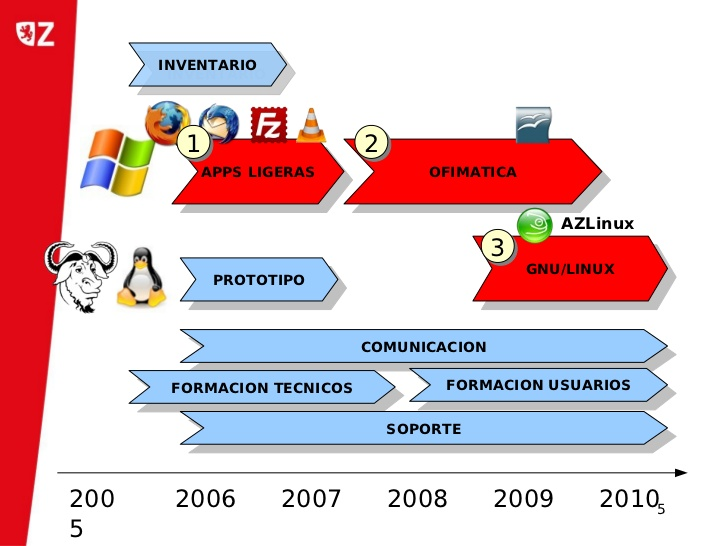
\includegraphics[scale=0.5]{img/desktopplan.jpg} 
  \caption[Migration plan in Zaragoza]{Migration plan for Zaragoza \protect\footnotemark}   
     \label {fig:plan-Zara}
     \end{figure}
     \footnotetext{ Source: \url{http://www.slideshare.net/eduromo/ubuntu-migration-at-zaragoza-city-council-v3}\label{planzaragoza}}
     
     \begin{figure}[H]
     \centering
         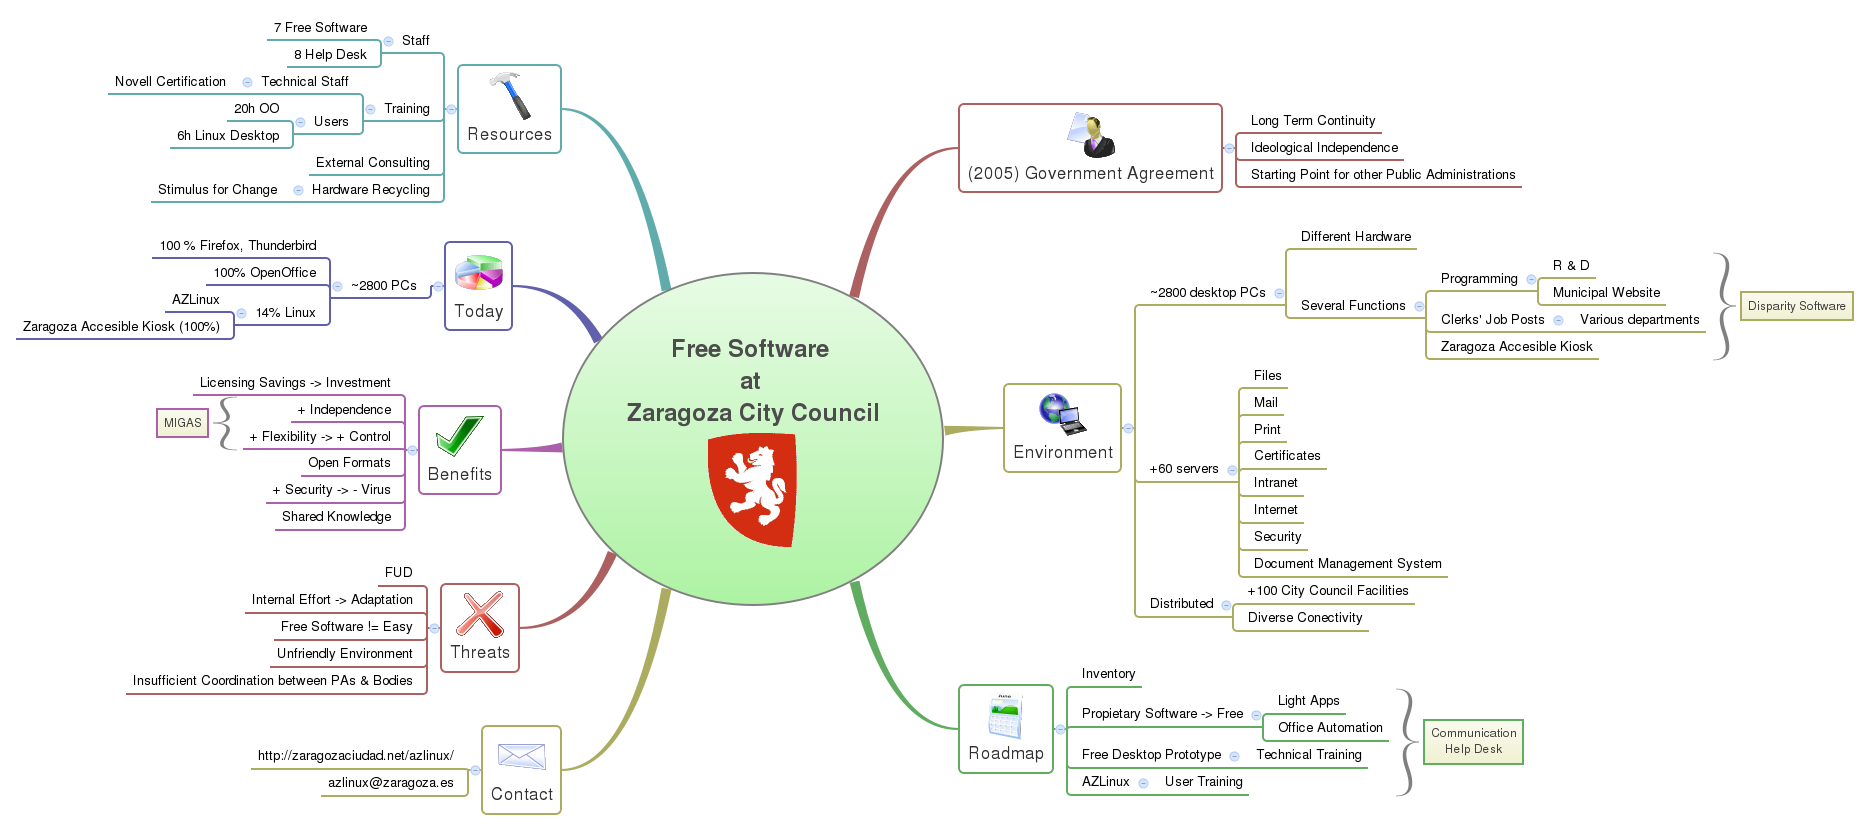
\includegraphics[scale=0.30,angle=90]{img/aytozgz.png} 
       \caption[Free Software at Zaragoza City Council]{Free Software at Zaragoza City Council \protect\footnotemark}
       \label{fig:FsZ}
         \end{figure}
     \footnotetext{Source:\url{http://www.zaragoza.es/contenidos/azlinux/gnome-marketing-hackfest\_2010-05-07.zip}}
     \newpage
\begin{itemize}
\item Phase 1: Lightweight Windows XP Applications – considered to be the easiest migration phase; with documentation and support from technicians, this phase was completed easily through the use of desktop applications in Windows XP. These applications included: the replacement of Internet Explorer with the use of Mozilla Firefox, the replacement of Outlook with Mozilla Thunderbird, the use of FileZilla as the primary FTP client, and the replacement of Windows Media Player with VLC.

  \begin{figure}
     \centering
         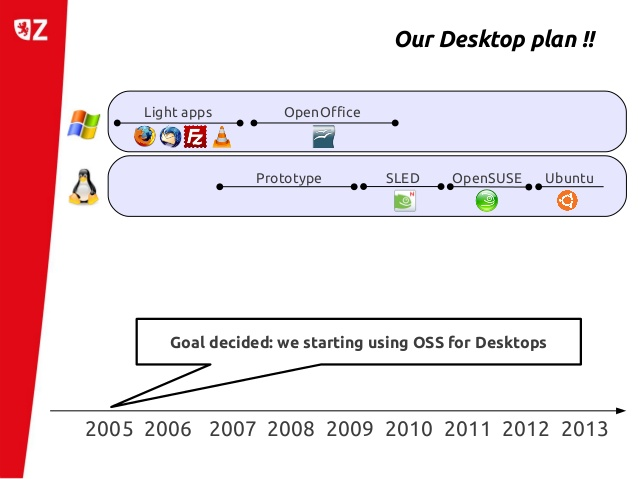
\includegraphics[scale=0.5]{img/zaragoza_desktopplan.png} 
       \caption[Zaragoza Desktop plan]{Zaragoza Desktop plan \protect\footnotemark}
         \end{figure}
     \footnotetext{Look at footnote \ref{planzaragoza}}


\item Phase 2: Office Applications – This phase allowed for the migration from Microsoft Office 97 to Open Office. The primary features in both office productivity suites are similar and contain similar functionality. There were issues present between MS Access and OpenOffice Database, given the fact that communication between the access documents was not possible; however, they were able to utilize Wine in GNU/Linux to complete the transfer. It was deemed the most important aspect of the migration process given the fact that all applications were utilized by all departments and the primary concern was not to interfere with the day to day operations of the departments, 
maintaining both quality and functionality. 
but recently they also started using LibreOffice, in combination with AZLinux12

\item Phase 3: Operating System – This phase consisted of the changeover in OS from Microsoft Windows XP to SUSE Linux Enterprise Desktop. Initially SuSE Linux Enterprise Desktop 10 was used in AZLinux 1, but this was changed to OpenSUSE 11.2 for AZLinux 2. SLED (SuSE Linux Enterprise Desktop) was the chosen application, given the fact that it had greater levels of integration with Novell Services (files, authentication, mail, etc.).
\end{itemize}
\textbf{Technical issues}
The city's IT department itself uses many more open source solutions, including for authentication (PAM\_LDAP), for digital certificates (FNMT) and for automatically migration tool to AZLinux (Win2Linux) and for system managemet they developed there own system (Migasfree)\footnote{Migasfree is a Repository Manager where you put packages to distribute. These packages are responsible for performing the software configuration change, and must be created by each organization. Written in the Python programming language and using the Apache web server.}

\subsection{Difficulties}
\begin{itemize}
\item Training gaps
It is hard to find qualified technicians in FLOSS in some specific field.
\item Low budget for additional costs, because there are costs associated with migration processes (training, acquisition of compatible hardware, etc.) these costs are not sufficiently understood.
\item Maintenance and Support. Many FLOSS projects implementation are carried out by individual initiative, without formal contracts to ensure their maintenance and support.
\item Lack of awareness of the importance of the FLOSS.
\end{itemize}


\subsection{Cost}
In total, the project is expected to save as much as 15 \% of the council’s total IT budget, demonstrating an effective use of tax-payers’ money to deliver better public services.

“\textit{ The new open source strategy will reduce our software licensing costs by 50 percent potentially saving as much as \euro.500,000  per
year compared with our previous Microsoft solution.”}\footnote{Ricardo Cavero,Science and Technology CEO
Ayuntamiento de Zaragoza}

\newpage

%---------------------------------------------------------------------------
\section {Munich ,Germany  }
\begin{figure}[H]
\centering
    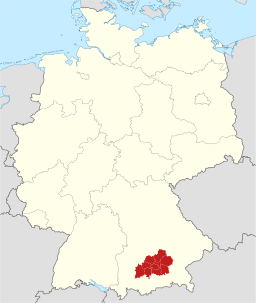
\includegraphics[scale=0.8]{img/munich.png} 
  \caption{ Munich City}
    \end{figure}

Munich, the capital of the federal state of Bavaria (Germany), has a population of approximately 1.23 million; it is the largest city in Bavaria and the third largest city in all of Germany, following on the heels of Berlin and Hamburg. The city of Munich has a network consisting of approximately 14,000 computers and approximately 16,000 users. The Linux distribution (distro) currently employed for a project sponsored by Munich’s city council is LiMux. The goal was total migration by January 2013 to free and FLOSS, allowing the city to achieve greater levels of independence from software distributors, client/server relations and native client software; the migration included more than 15,000 personal computers (PCs) and laptops of the city’s various public employees.

\subsection{The plan}
The goals of the city council included:
 \footnote{\url{https://joinup.ec.europa.eu/elibrary/case/limux-it-evolution-open-source-success-story-never}}
\begin{itemize}
\item FLOSS, including the use of office communication software based on open standards, for all desktop PCs in the municipality,
\item The ability to make, develop, and/or procure all administrative processes as platform-independent software,
\item The creation of a standardized IT platform that included all consolidated applications and data storage.
\end{itemize}
The migration process started in 2004 with the introduction of four specific goals for IT administrators:
\begin{enumerate}
\item The migration of all desktops from the Windows OS to the LiMux OS.
\item The migration of specialized administrative processes to the use of free, web-based, or native Linux solutions.
 \item The reduction of complexity through the consolidation of the number of software products utilized.
\item The transference of macros, templates, and forms to the new solution, introducing system management software deployment and a centralized sign-on process. 
\end{enumerate}
%---------------------------------------------------------------------------
\subsection{Training and  E-learning }
At the start of any migration, it is typically the department administrators that will need additional training, providing them with the opportunity of learning how to deploy and run the new software options. After the administrators and technical staff have received their training, it is then typically the responsibility of the project team to create an e-learning environment, one that will teach others about how to utilize the software. In this instance, the project team created “LiMux Lemwelt” (the LiMux learning world), allowing users to take advantage of the entire experience, providing users with the freedom to choose the different areas and software products that they wished additional training on, while allowing users to control the pace of their training. In 2007, the LiMux Lemwelt received the eurele, a European e-learning award, for its design and functionality. Workers who utilize this program were trained only when their specific area was up for migration, allowing them to smoothly transition, seamlessly applying what they learned within the training sessions to the real world setting.
\begin{figure}[H]
    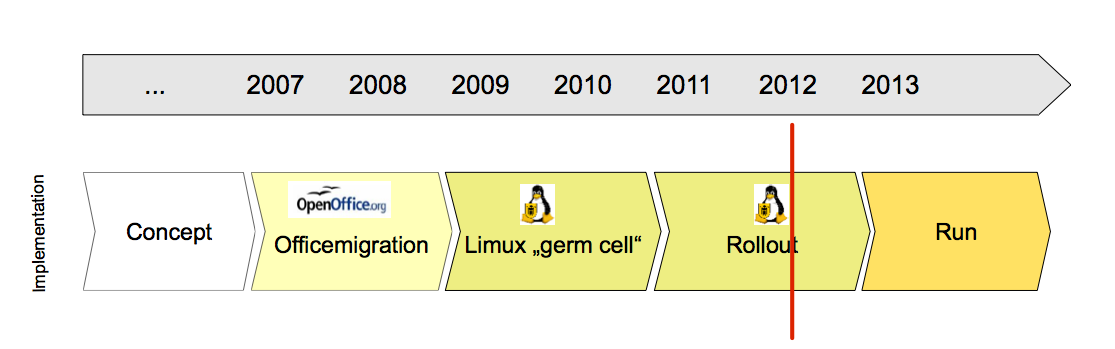
\includegraphics[scale=0.4]{img/timeline_limux.png}
 \caption  [Limux Timeline]{Limux Timeline © LiMux Project}  
\end{figure}
The timeline determined for the implementation of this process was as follows:
\begin{itemize}
%---------------------------------------------------------------------------
\subsection{Timeline}

\item 2001–2003: First plans and discussions based on the results of the city council of Munich votes.
\item 2003: project started.
\item 2005: The LiMux project started officially converting PCs.
\item 2008/2009: The first step, the complete switch to OpenOffice.org enabling the Open Document Format as standard format is done.
\item Late 2012: Initial goal of 12,000 Linux-based machines achieved.
\item  2013: Final acceptance documents signed, regular operations mode started, 14,800 machines migrated to Ubuntu Linux and LibreOffice.
\item December 2013: Munich open source switch completed successfully.

\end{itemize}
%---------------------------------------------------------------------------
\subsection{Cost}

Munich’s decision to leave Windows behind as their preferred and primary OS was not financially motivated, in spite of the fact that Munich indicated that the move to FLOSS allowed the city to save more than \$10 m . In total, the LiMux project cost  \$23 m , as compared to the original  \$34 m  that was estimated it would cost to stay with Windows and MS Office. While HP created a report on behalf of Microsoft, that argued that the shift to FLOSS would cost three times as much as the official figures indicated, officials in Munich were able to show that the report was based off of a variety of flawed assumptions, among them being the overestimation of the number of staff it would take to accomplish the task.

 \begin{figure}
 \centering
     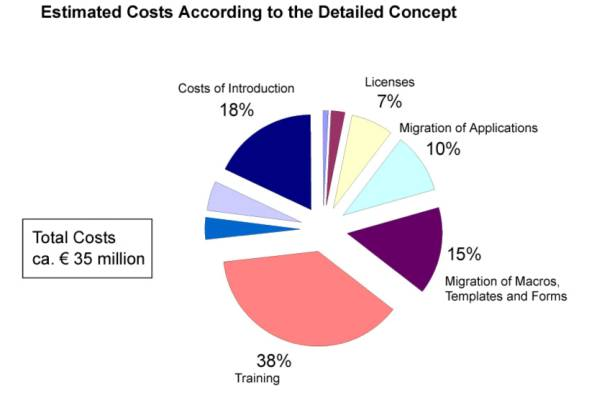
\includegraphics[width=0.86\textwidth]{img/cost_limux_estimates.png}
   \caption  [Limux cost estimates]{Cost Estimates According to the Detailed Concept \protect\footnotemark}  
   \label{fig:cost_limux_estimates}
 \end{figure}
 \footnotetext{source:\url{http://waste.informatik.hu-berlin.de/grassmuck/texts/limux.pdf`} }

Through a review of Figure \ref{fig:cost_limux_estimates}, it is possible to see that the final cost associated with training is the highest conceptualized cost estimate, according to LiMux – Free Software for Munich. 

\textit{“By combining the low costs and freedom of open source software with ongoing support for the hardware and applications we need, it was one of the critical elements to the success of this project. Most important was the backing of our politicians throughout the project.”}\footnote{Peter Hofmann, project manager for the City of Munich in \url{https://insights.ubuntu.com/2014/07/07/ubuntu-and-open-source-help-the-city-of-munich-save-millions/}}

\begin{figure}
\centering
    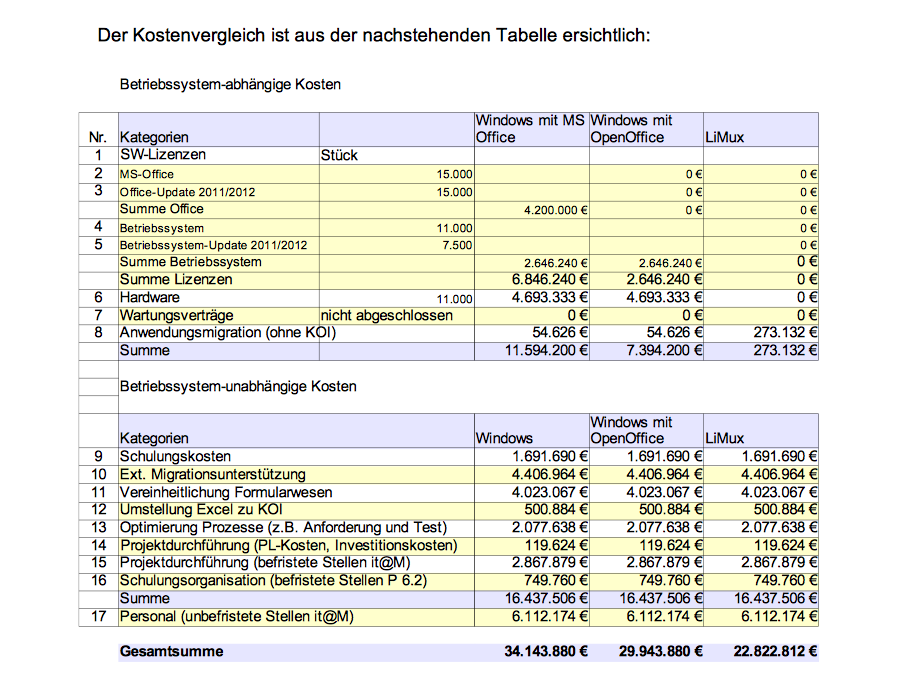
\includegraphics[scale=0.55]{img/limuxcost.png}
  \caption [Limux detailed cost]{Detailed figures of the LiMux project reveal differences from the original plan. Despite the economic success of LiMux, money has never been the driving factor. © Limux } 
\end{figure}
%---------------------------------------------------------------------------
\section {Largo ,Florida}
\label{largo}
\begin{figure}[H]
\centering
    \includegraphics[scale=0.8]{img/Largo.png} 
  \caption{ Largo Florida City}
    \end{figure}
Largo is the third largest city in Pinellas County, Florida, USA.
The city of Largo has a population over 70,000 with over 650 employees utilizing FLOSS including the use of the Linux OS and many other FLOSS options. The initial migration to the use of FLOSS started with 650 employees being selected to utilize the new system. Starting in 1993, Largo implemented the use of a thin client, thick server architecture, accessible from 425 thin client workstations.

As the use of Microsoft Windows was considered expensive to purchase and maintain, Largo chose to implement a migration and upgrade strategy that utilized graphical workstation environments with thin client devices. The Largo architecture was running on open server and UnixWare. 

In 2000, problems and difficulties started to arise at the Santa Cruz operation\footnote{Santa Cruz Operation (SCO) was a software company based in Santa Cruz, California which was best known for selling three Unix variants for Intel x86 processors: Xenix, SCO UNIX (later known as SCO OpenServer), and UnixWare.}, the provider of the Open Server and UnixWare, the initial reason behind the decision of the Largo IT staff to start the replacement process. At this same time, Microsoft had just come out with Windows 2000, an OS that was full of bugs and difficult to maintain, not to mention highly costly; as an alternative, Largo chose to utilize Red Hat Inc.’s Linux Server options instead. The project started with 20 employees test running the new environment, and by the middle of 2001, Largo’s IT team was satisfied with the results.

\subsection{FLOSS and Largo’s needs.}

 Largo’s environment serves 650 user accounts on a network of 400 computer devices. This network is served by two Compaq servers, with each server supporting approximately 220 users. KDE desktop environments are utilized by Largo’s staff. Opera and Netscape are the web browsers of choice, with Ximian based on the GNOME platform used as the primary email client, and Apache servers being utilized as additional application support.
 
  Largo’s IT team succeeded in their experiment, but they believe that the primary barrier to greater acceptance of the use of FLOSS is the unbelieving nature of many that the software options are equal to or better than standard licensed programs.

\paragraph{Training users on Linux}
One of the biggest problems training new employees to switch from Windows PCs, to use Largo's Linux-based network. 
They are used to system crashes and network failures in Windows environments that they have trouble realizing, that all their files are stored on reliable servers -- with backups -- instead of on a desktop PC.

\textit{"There is also another, very human problem to overcome: that most people don't understand computers or software, but have memorized all the keystrokes and mouse-click patterns they need to get through the day, so the second they are given a new program they need to memorize a whole new set."}\footnote{\url{http://www.largo.com/eGov/apps/document/center.egov?view=item;id=1793}} This can happen any time when new software is introduced in a workplace environment. But train people and answer users' questions will help new users to overcome this difficulties.

\subsection{Cost}
Systems administrators in Largo estimated that the use of Linux saves the city approximately \$1 m per year in hardware, software licensing, maintenance, and staffing costs, as of 2002. The IT staff looked at the possibility of continuing to utilize Microsoft Office, but ultimately decided that the total cost of installation, licensing, and maintenance could easily hit \$1.5 m over the course of a six year cycle, while the maintenance of OpenOffice during the same period would be roughly \$100,000 .\footnote{Look at the previous footnot} 
The cost differentiation between the two programs is shown below in Figure ~\ref{fig:Largo_cost} 
\begin{figure}
\begin{center}
    \includegraphics[scale=0.9]{img/largocost.png}   
\end{center}
 \caption[Largo Office Cost ]{Total Cost of Installation, Licensing, and Maintaining the Different Productivity Suites for a 6-year Cycle}
    \label {fig:Largo_cost}

\end{figure}



\newpage
\begin{savequote}[108mm]
 " Don't mistake activity with achievement."
   \qauthor{John Wooden}
\end{savequote}
\chapter{Conclusions}
\label{chap:conclusions}
\vspace{-2cm}

This research explored the advantages and challenges that are faces by organizations who want to migrate to FLOSS. One reason found for wanting to migrate to FLOSS is for cost savings. The research found that there are many hidden costs and challenges that must be faced in the migration of the software. Understanding scope of the migration process and the needs of the organization are the most important consideration in a successful process. FLOSS can add complexity to an existing system. Compatibility issues are one of the challenges that were found to be a determining factor in the success of the migration process. 

One of the most important considerations to the success of the migration project is providing support for users during and after the implementation process. Because the software itself is not owned by a single corporation, the company no longer has the option of calling the software developer to fix the system or to offer support when it breaks. This is the reason why setting up an in-house support system is an essential part of the success of the migration. Employees must have someone they can call when they have questions or problems. 

It is recommended that government entities have an obligation to exercise oversight of public resources to the greatest extent possible. This means implementing cost saving solutions wherever possible. FLOSS was found to save considerable costs both in the short and long term. There are no more licensing fees, and one does not have to pay to expand the system and add more users. The flexibility of FLOSS is another feature that makes it an excellent choice for organizations and government entities. This opinion is supported by the numerous successes found in the case studies used in this research. 

\section{Evaluation}
The goal of this research was to explore the FLOSS migration in government and private organizations. In meeting that goal, several case studies were found that provided a framework for the development of a migration plan that will be useful in majority of the cases involved in a migration from CSS to FLOSS. This research was successful in exploring the advantages of migrating to an FLOSS system. It also explored the challenges and developed a plan that will result in attention to the major areas that were found during the case study review.

The case studies identified supported the premise of the study and the advantages of FLOSS for government entities. It sufficiently addressed the intended answers that it hoped to find. The research demonstrated that although cost is a fact in the decision to migrate from CSS to FLOSS, this not the only factor that is considered. Outpacing cost as a reason for migrating to FLOSS, the organization has the freedom to design a system that specifically meets their needs. When one purchases CSS, they are getting a prepackaged  software, it will often have things that they do not need, yet be lacking in the features that they do need. FLOSS gives companies the freedom that they need to design a system that is the perfect fit.          
%----------------------------------------------------------------------------------------------
\section{Lessons learned}
\label{sec:lessons}
Several lessons were learned throughout the course of this research study. 
\begin{itemize}[itemsep=0ex]
\item  The first lesson is that is not only possible, but necessary for government entities to take advantage of the savings and flexibility that FLOSS has to offer.
\item It is necessary to convince people to be ready and open for change.
\item One of the key goals of the migration process is to make the transition from proprietary software to FLOSS as seamless as possible. The goal is to make the change without sacrificing business continuity. Compatibility issues can bring the business to a halt during the migration process. This can cost the company untold losses in terms of monetary losses.
\item The critical phase of the migration plan is to determine the needs of the organization and to set measurable goals for completion of the project.
\item Planning is the most important phase of the migration process.

\end{itemize}

In a personal aspect through conducting this study, gaining the knowledge and skills necessary to successfully implement the migration from CSS to FLOSS. having the ability to plan and execute a migration plan. Familiar with the challenges and obstacles that could be faced in the implementation and execution of the project. 
This research provided me with the opportunity to expand my knowledge and skills in the area of software migration and FLOSS for small, medium, and large government entities.
\subsection{Knowledge and Skills Acquired }
The following explains knowledge and skills acquired in the M.Sc. studies that helped me on
this work:
	\begin{enumerate}[itemsep=0ex]
	
\item \textbf{Introduction to Libre Soft.}

 This course explored the fundamentals of Libre Software and its history and evolution. This research project added to the knowledge learned in class through allowing me to explore how it is used in real world applications.

\item \textbf{Legal Aspects of Libre Software.} 

This course explored the legal aspects of Libre Software including copyright, licensing, patents, lawsuit, and other legal issues. This course helped me to understand the types of issues involved when choosing an FLOSS licensing. 

\item \textbf{Economic Aspects of Libre Software.}

 This course explored the economic motivations behind FLOSS. This course played an essential role in helping to build the case for encouraging organization to begin using FLOSS. Although the economics are an important part of the motivation to switch, it was found that other factors, such as the ability to design a customer system to meet their needs. This turned out to be more important than the economic reasons for the switch. 
 
\item  \textbf{Case Studies.}

Thanks to this course I met \textit{Eduardo Romero}, Computer technician at City of Zaragoza. He inspired and encourage me to do this work, his speech was helpful for me to do this work. and I am looking forward to move his experience back home. 
                 
   \item \textbf{Developers and Motivation of LibreSoft.}
                 
 This course taught me the motivations of libre software developers, roles and organization in libre software projects and the leadership in libre software projects. Much of the information obtained in this course was be applied when studying the migration motivation and plans, and how to lead and organize the migration.
 
 \item \textbf{System Integration. }
 
 This course provided information on system platforms, virtualization, and network administration of FLOSS. This course was valuable in helping me to identify and foresee challenges that could occur during the migration.
 
\item \textbf{Project Management }

This course provided me with the knowledge to break the task down into manageable phases to be carried out. It was inspiration for the organization of the migration process. for instance documentation and communication channels can be good way for reaching new contributors and stability of the projects. 

\item \textbf{Project Evaluation of Libre Soft, Development Tools of Libre Soft.}

These courses taught me to take into account every aspect of the software beyond the code or how it works. I found out how to use the control version system that I used to keep track of each change made to this document. This project made me look at the impact of the software on the organization as a whole. It made me look at the bigger picture beyond the code.  I also learned the importance of FLOSS project evaluation, which I was able to apply in the development of the migration plan. 

\item\textbf{ Advanced Development. }

This class taught how to make Android software. This course  provided me with background on some of the compatibility problems that may be encountered when transferring between platforms.          

                                                                                               
	\end{enumerate}
\section{Future work}
\label{sec:future}
In the future, this work will continue through seeking out more case studies so that the experience can be added to the overall knowledge on the topic. The more case studies that are read, the broader the knowledge base will be and the easier it will be to apply that knowledge to the more migration projects. Case studies provide examples and insight as to how to overcome challenges that may arise. 

In addition to finding more case studies and increasing the knowledge base, the researcher will provide a specific plan for a migration. The researcher will then attempt a migration to FLOSS. This future work will provide practical field experience and the ability to see what types of issues arise that were not discovered as part of this research study.  Finally, future research will entail a comparison of different types of FLOSS that provide the best migration experience. This will help organizations to choose the right FLOSS for their migration.                                                                                                                                                                                                                                                                                                                                                                                                                                                                                                                                                                                                                       




%----------------------------------------------------------------------------------------------
\appendix

\chapter{Acronyms} 
\label{apn:Acronyms}
\vspace{-3cm}
\begin{acronym}
\acro{CSS}{Closed-Source Software}
\acro{EULA}{End user License Agreement}
\acro{FLOSS}{Free/Libre and Open Source Software}
\acro{FOSS}{Free and Open Source Software}
\acro{FSF}{Free Software Foundation}
\acro{GNU}{GNU is Not Unix}
\acro{ICT}{Information and communications technology}
\acro{NSA}{National Security Agency}
\acro{OS}{Operating System}
\acro{OSS}{Open Source Software}
\acro{OSS/FS}{open source software and free software}
\acro{SELinux}{Security-Enhanced Linux}
\acro{TCO}{Total Cost of Ownership}
\end{acronym}


%----------------------------------------------------------------------------------------------
% BIBLIOGRAPHY %
\nocite{*}
\bibliographystyle{abbrv}
\bibliography{bibliography}
\label{Bibliography}

%----------------------------------------------------------------------------------------------

\end{document}
